\graphicspath{{images/chapter1/}}

\chapter{Literature study}
\label{chap:rel_work}
In order to correctly implement a solution, we need to first understand the fundamentals.
These consist of two research fields: HPE and \gls{NST}.
The former will be used to detect poses in the art collections, but not before the latter has tried to make an improvement.
Following will be an overview of the available research in these domains.
Discussing what the goals of them are, how they achieve it, what their challenges are and their limitations.

\section{Generative Adversarial Network}
\glspl{CNN} have become the default go-to for many visual tasks and, in order to train a CNN correctly, it needs to minimize a loss function.
This is something that still requires a great amount of effort in manually crafting loss-functions.
For example, when using Euclidean distance to calculate loss during image generation, it will create a network that outputs blurry images, as minimizing Euclidean distance is achieved by averaging the output.
Having a loss-function that does what it should is a difficult problem to solve.
To sidestep these complications, Goodfellow et al. \cite{Goodfellow2014} propose a framework where the generative model competes against a discriminative model that learns to make a distinction between a sample from the real distribution and one from the generative model's distribution.
Figure \ref{fig:generative_adversarial_network} shows the architecture of a \gls{GAN}.
It consists of a generator $G$ which takes in random noise and attempts to output a sample from a specific distribution.
The discriminator $D$ will then try to distinguish between the sample from the generator and a real sample from that distribution.
A popular variation of \gls{GAN} is the \gls{cGAN}, this architecture feeds an extra label to the generator and discriminator, so that it can be conditioned to generate certain images based on the label.

\begin{figure}[h]
	\centering
	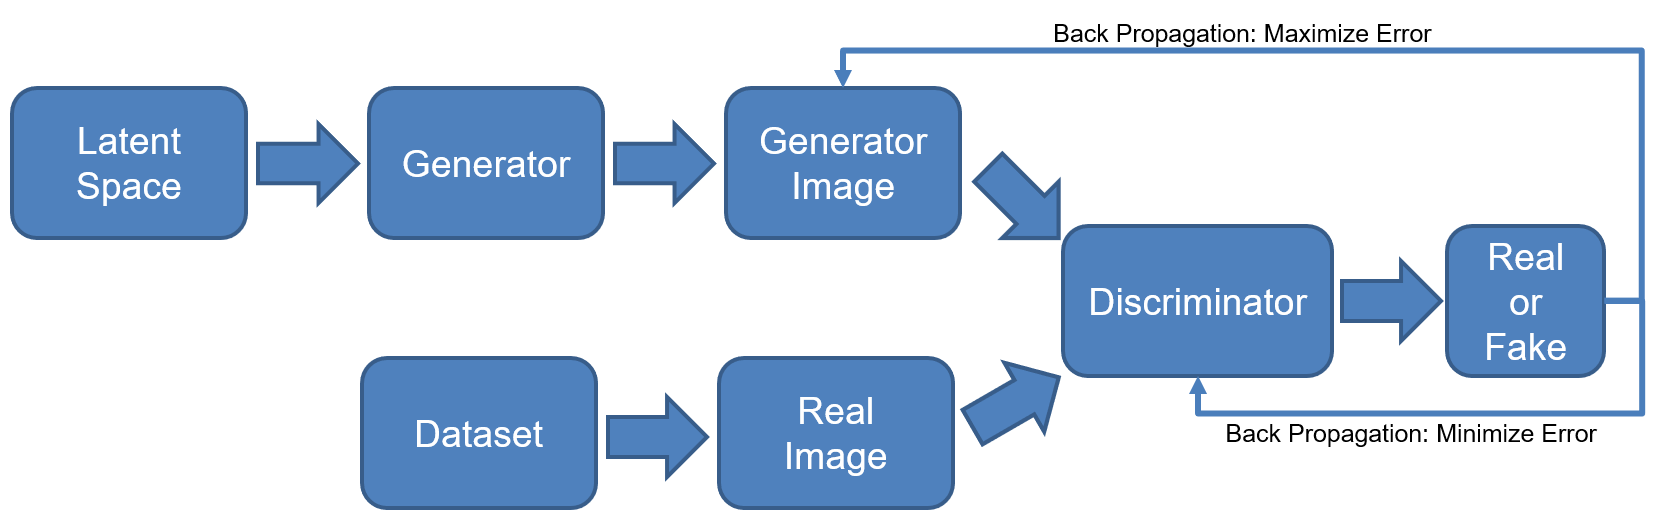
\includegraphics[width=0.8\textwidth]{generative_adversarial_network}
	\caption{The architecture of the Generative Adversarial Network \cite{GANCookbook}.}
	\label{fig:generative_adversarial_network}
\end{figure}

\section{Human Pose estimation}
\label{sec:hpe}
HPE aims to detect human features from input data such as images and videos.
It's an elementary part of computer vision with many applications among which are human action recognition (sign language), human tracking (surveillance), and human-computer interaction (video games).
This is an extensively researched area with a diverse range of different techniques.
This chapter will give an overview of all the many challenges and proposed solutions.
The focus will be on deep learning models, which have surpassed classical solutions significantly.
Specifically, around 2D HPE \cite{Munea2020, Zheng2012, Liu2104, chen2022}.

\begin{figure}[h]
	\centering
	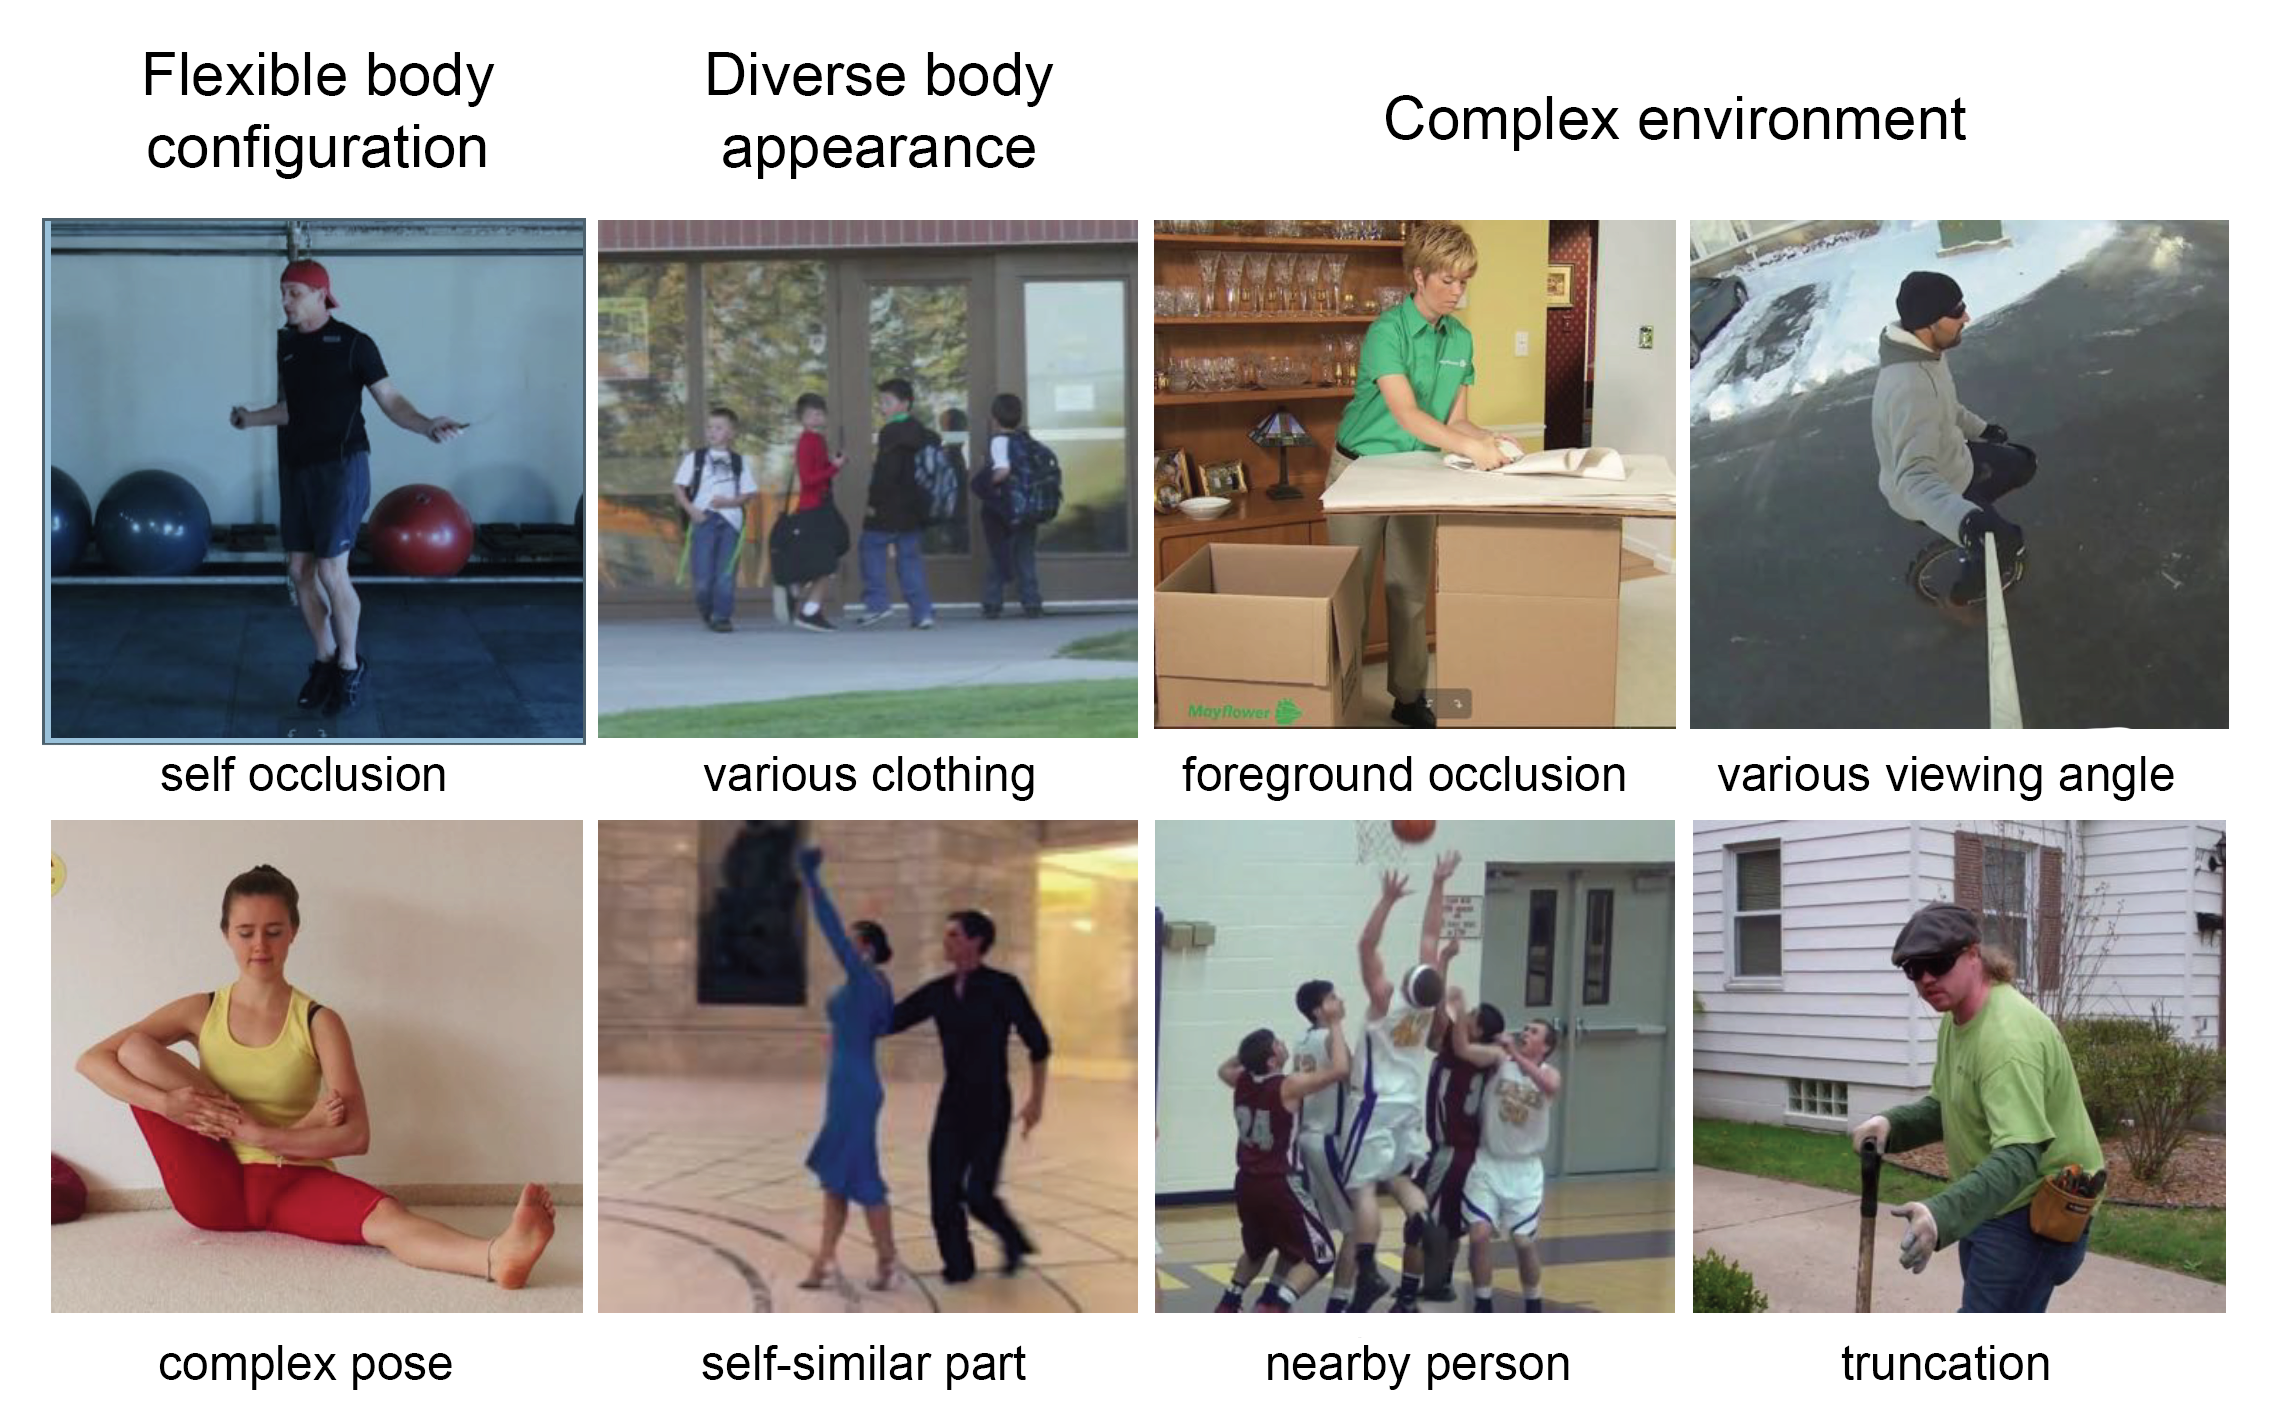
\includegraphics[width=0.6\textwidth]{hpe_problem_complexity}
	\caption{The various challenges HPE solutions face. Images from \gls{MPII} dataset. \cite{Andriluka2014, Chen2000}}
	\label{fig:hpe_problem_complexity}
\end{figure}

The human body has a high degree-of-freedom due to all the limbs, self-similar parts and body types, which may cause self-occlusion or rare/complex poses.
The variations in configuration are made even larger due to clothing, lighting, foreground occlusion, as well as viewing angles and truncation, among others.
Examples of this complexity are shown in Figure \ref{fig:hpe_problem_complexity}.
This makes HPE one of the most difficult tasks in computer vision \cite{jain2014, Chen2000}.

\begin{figure}[t]
	\centering
	\subcaptionbox{Skeleton \label{fig:pose_representation_skeleton}}{%
		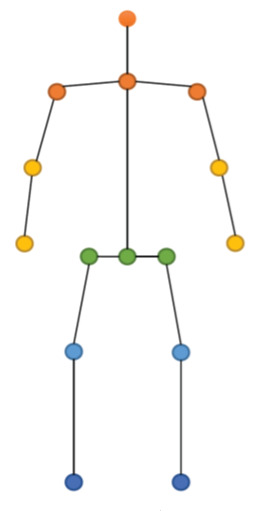
\includegraphics[width=0.15\textwidth]{pose_representation_skeleton}%
	}
	\subcaptionbox{Contour \label{fig:pose_representation_contour}}{%
		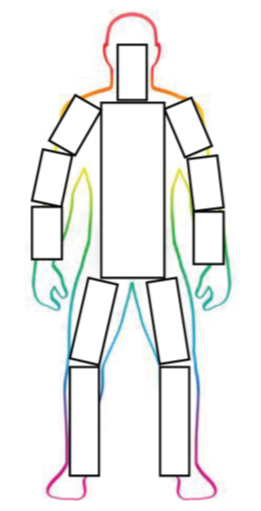
\includegraphics[width=0.15\textwidth]{pose_representation_contour}%
	}
	\subcaptionbox{Volume \label{fig:pose_representation_volume}}{%
		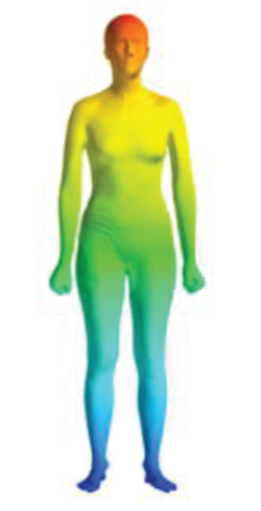
\includegraphics[width=0.15\textwidth]{pose_representation_volume}%
	}
	\caption{Models for pose representation \cite{Zheng2012}}
	\label{fig:pose_representation}
\end{figure}
\subsection{Representation}
\label{section:representation}

An important factor in HPE is how the pose will be represented.
Depending on the needs of the problem you can have a skeleton-based, contour-based, or volume-based solution \cite{Chen2000} as seen in Fig. \ref{fig:pose_representation}.

\subsubsection{Skeleton-based model}
The skeleton is made of a tree-structured set of keypoints that represent the joints of the human body.
These can be explicitly described by their coordinates in 2D or 3D space \cite{Toshev2014}.
More suitable for a CNN, however, is a heatmap which constructs a 2D Gaussian kernel around a keypoint \cite{Liu2104, SWARH}.
As they are easily implemented, they became the dominant representation.
While the skeleton-based model is a compact and flexible representation, it suffers in this aspect by not being able to hold texture or shape information \cite{Zheng2012}.

\subsubsection{Contour representation}
To capture the shape of the body parts, contour representation uses rectangles to estimate the body contours.
These methods include cardboard models \cite{Ju96}, which assumes people can be represented as a group of planar patches, and Active Shape Models \cite{COOTES95}, which tries to fit body part shapes to an image.
They were used in earlier HPE methods \cite{Chen2000}.

\subsubsection{Volume representation}
Volumetric geometric shapes can also be used as a method of representation.
Earlier methods used simple shapes like cylinders, conics, and other shapes \cite{Sidenbladh2000}.
Volume representation is a 3D mesh that represents the human body.
The most used model is Skinned Multi-Person Linear, which includes natural pose-dependent deformations imitating soft-tissue dynamics \cite{Loper2015}.  
\\
\\
For the purpose of this research, a simple model is more than adequate.
Only the most essential joints are needed to label a pose.
This makes the skeleton-based model the ideal representation to work with and will be the focus of further study.

\subsection{Datasets}
There are several publicly available datasets.
Some are outdated and will be left out, focusing only on datasets used for deep learning.

\begin{enumerate}
	\item \textbf{\gls{LSP} Dataset \cite{Johnson2010}} contains 2,000 images found on Flickr using 8 different tags looking for sport activities (athletics, badminton, baseball, gymnastics, parkour, soccer, tennis, and volleyball).
	Each person has 14 keypoints.
	An extended version was later introduced \cite{Johnson2011}, now consisting of 10,000 images. 
	For this set, they only focused on the more challenging tags (parkour, gymnastics, and athletics).
	\item \textbf{\gls{MPII} Human Pose Dataset \cite{Andriluka2014}} contains 24,290 images with 40,522 labeled people.
	They were extracted from YouTube videos found by querying for physical activities.
	Each person has 16 keypoints and it also includes occlusion labels.
	\item \textbf{\gls{COCO} Dataset \cite{Lin2014}} is a large-scale dataset for a wide range of computer vision algorithms.
	For HPE, the set contains more than 200,000 images in which 250,000 persons are annotated.
	Each person has 17 keypoints, a bounding-box and visibility labels.
	This dataset has become the most popular for benchmarking.
	\item \textbf{\gls{FLIC} Dataset \cite{Sap2013}} contains 5,003 images extracted from Hollywood movies.
	They ran a person detector which collected 20,000 images from 30 movies.
	Occluded and difficult poses were then removed leaving only 5,000 images to be annotated.
	Only the upper body received 10 keypoints.
	\item \textbf{\gls{AIC-HKD} Dataset \cite{Sap2013}} contains 300,000 images found using Internet search engines.
	In these, over 700,000 humans are annotated.
	Each person has 14 keypoints, a bounding-box, as well as visibility and left/right labels.
	\item \textbf{CrowdPose Dataset \cite{Li2018}} puts an emphasis on crowded images.
	30,000 images from \gls{MPII}, gls{COCO} and gls{AIC-HKD} were measured with a Crowd Index, which evaluates the crowdedness.
	Finally, 20,000 images are selected and 80,000 persons annotated.
	Each person has 14 keypoints and a full-body bounding box.
	\item \textbf{Human-Art Dataset \cite{Ju2023}} bridges the gap between natural and artificial images.
	The set contains 50,000 high-quality images with 123,000 annotated humans.
	Each person has 17 keypoints, bounding boxes, self-contact points, and text information.
\end{enumerate}

\subsection{Discriminative Methods and Generative Methods}
Before deep learning became prominent in HPE, there were already a number of different methods in use.
Some of these methods are compatible with the deep learning methods and were promptly adopted.
An early distinction is between generative and discriminative methods.

\textbf{Generative Models} work with prior beliefs about the pose.
More information about this can be found in the section about representation \ref{section:representation}.
It will project the pose on the image and verify it with the image data.
If it doesn't comply, the pose is adjusted using descent directions found by minimizing an error function to converge to a local optimization \cite{Pons-Moll2011}.

\textbf{Discriminative Models} on the other hand, try to map the pose on the image data with learned models.
There are several methods in this category, among which are the deep learning-based methods.
The deep-learning methods are further categorized by the following sections.

\subsection{Single-Person Pose Estimation Methods}
Single-person pose estimation tries to evaluate only one pose from an image.
There are two major methods that are in use: regression methods and detection-based methods.

\textbf{Regression-based Methods} learn a network that maps all the body keypoints to the image directly, as shown in Figure \ref{fig:single_pose_estimation_regression_methods}.
The first successful deep learning model came from Toshev and Szegedy \cite{Toshev2014} and is considered the switch in paradigm from classic approaches to deep learning HPE.
Based on AlexNet for its simple but effective architecture \cite{AlexNet}, they use a seven-layered model with five convolution layers and two fully-connected layers for the pose regressor.
They then cascade the resulting found keypoints to the next stage where it refines it using the area around the keypoints.
While the network is the same, the different stages will have different learned parameters.
With every stage, the found keypoints become more accurate.
Carreira et al. \cite{CarreiraAFM15} introduce an Iterative Error Feedback which is a self-correcting model using top-down feedback.
Using the image and a starting pose modeled as a heatmap, the model, based on GoogLeNet \cite{googlenet}, will predict an error for each keypoint.
The pose is then corrected based on the error and fed into the next module as a heatmap with the input image.
With each iteration it converges towards the solution instead of making the prediction in one go.
Regression-based methods map the keypoints directly on the image, making it a non-linear problem, which leads to a less robust generalization \cite{Liu2104}.

\begin{figure}[h]
	\centering
	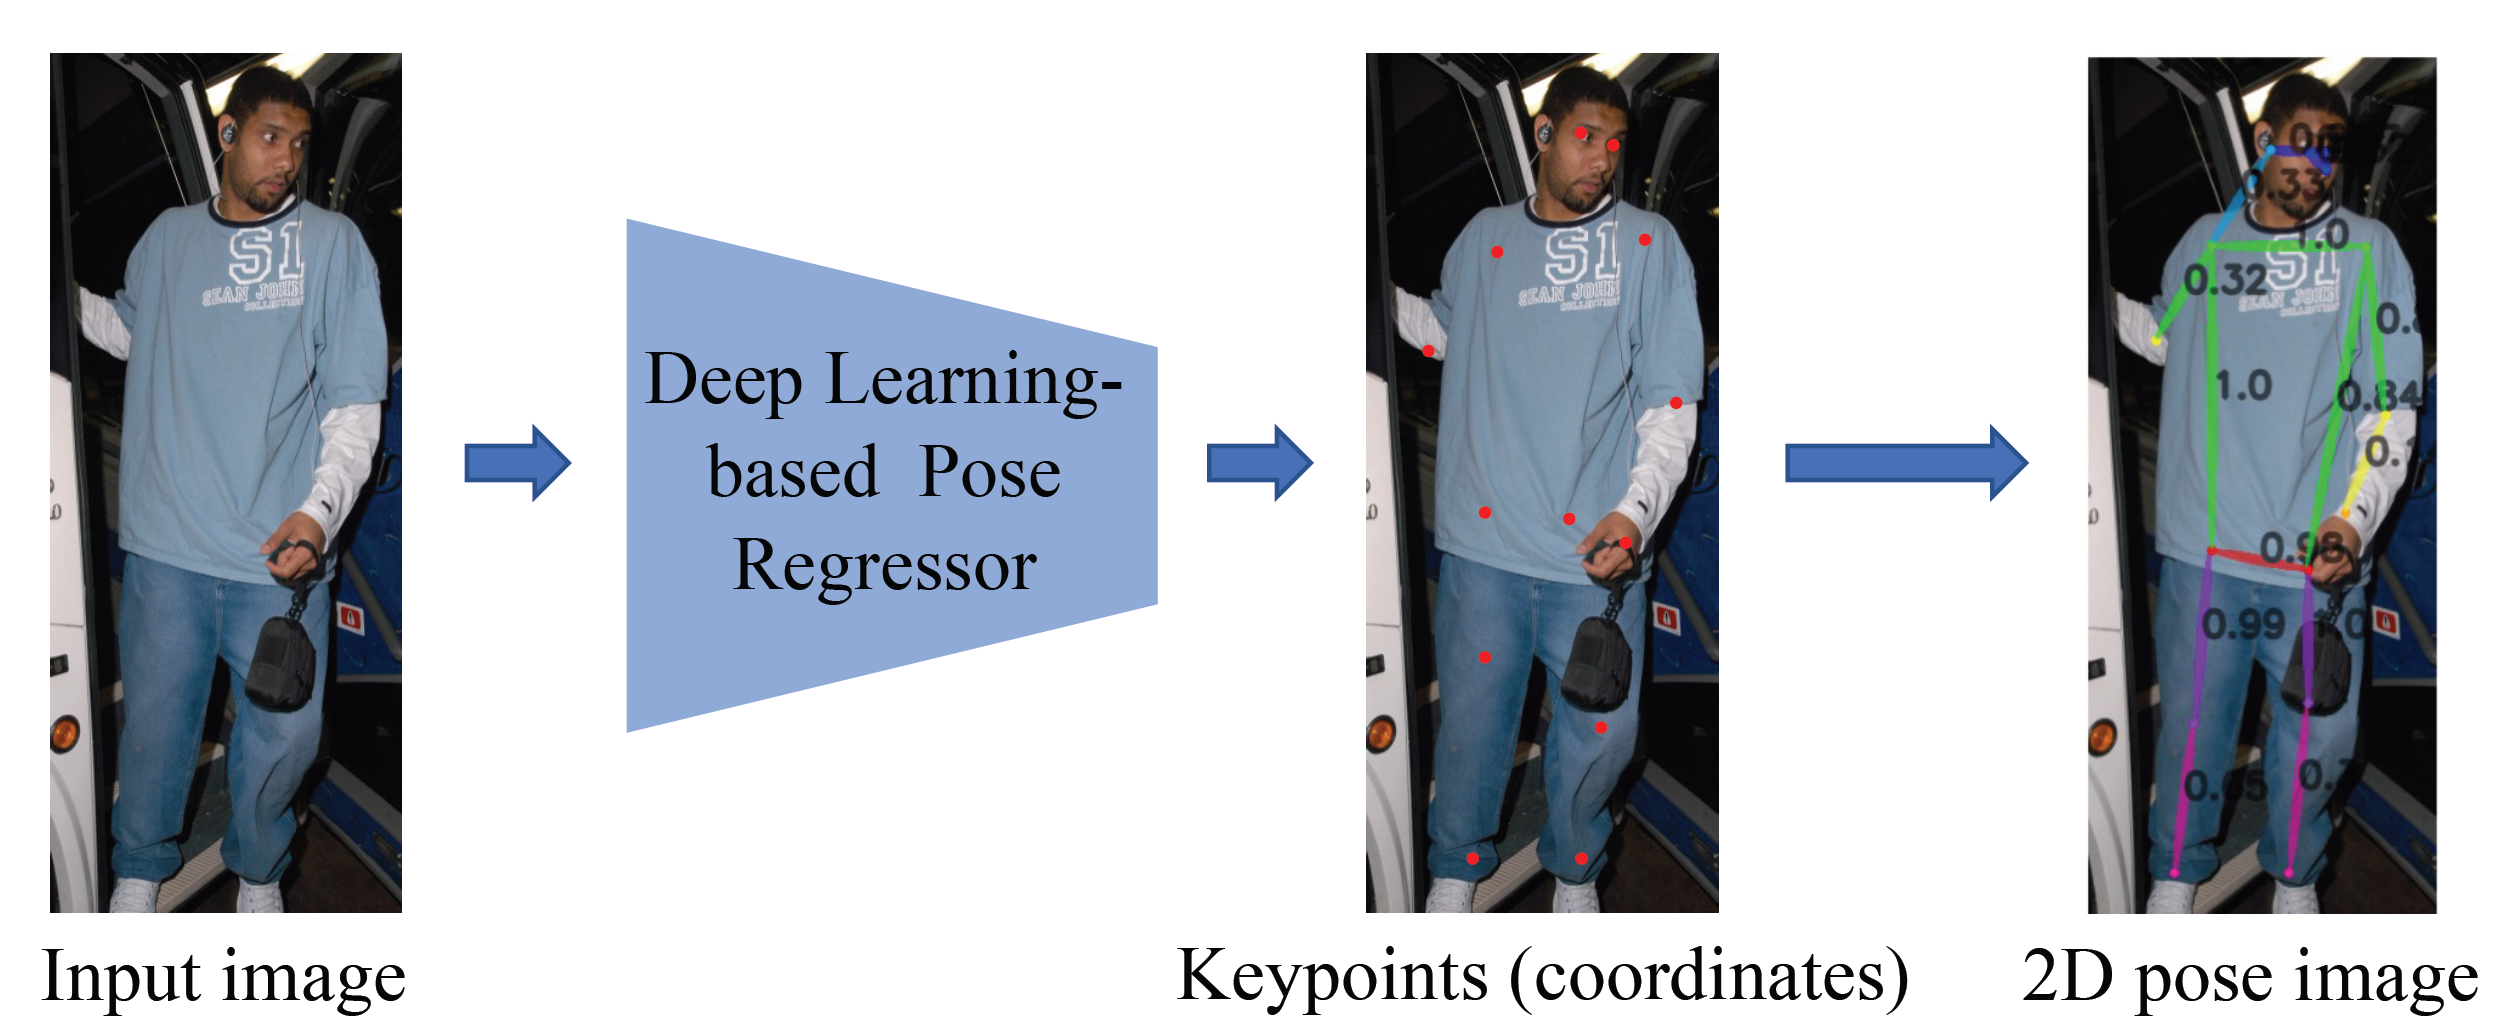
\includegraphics[width=0.6\textwidth]{single_pose_estimation_regression_methods}%
	\caption{Single-Person HPE Regression Methods as presented in \cite{Zheng2012}}
	\label{fig:single_pose_estimation_regression_methods}
\end{figure}

\textbf{Heatmap and Detection-based Methods} will first estimate the individual body parts using heatmaps.
This method results in an easier optimization and a more robust generalization \cite{chen2022}.
Most of the latest HPE methods use heatmaps because of this.
After the joints are found, they are assembled to fit a human skeleton, as shown in Figure \ref{fig:single_pose_estimation_heatmap-based_methods}.
Tompson et al. \cite{TompsonJLB14} proposed a hybrid architecture where the detection of body parts is handled by a CNN and a Spatial-Model to bring those together.
The first step produces many false-positives which are removed in the second step by restricting joint inter-connectivity to enforce correct anatomy.
They build on this in \cite{Tompson2015} where they use a cascade to refine predictions.

\begin{figure}[h]
	\centering
	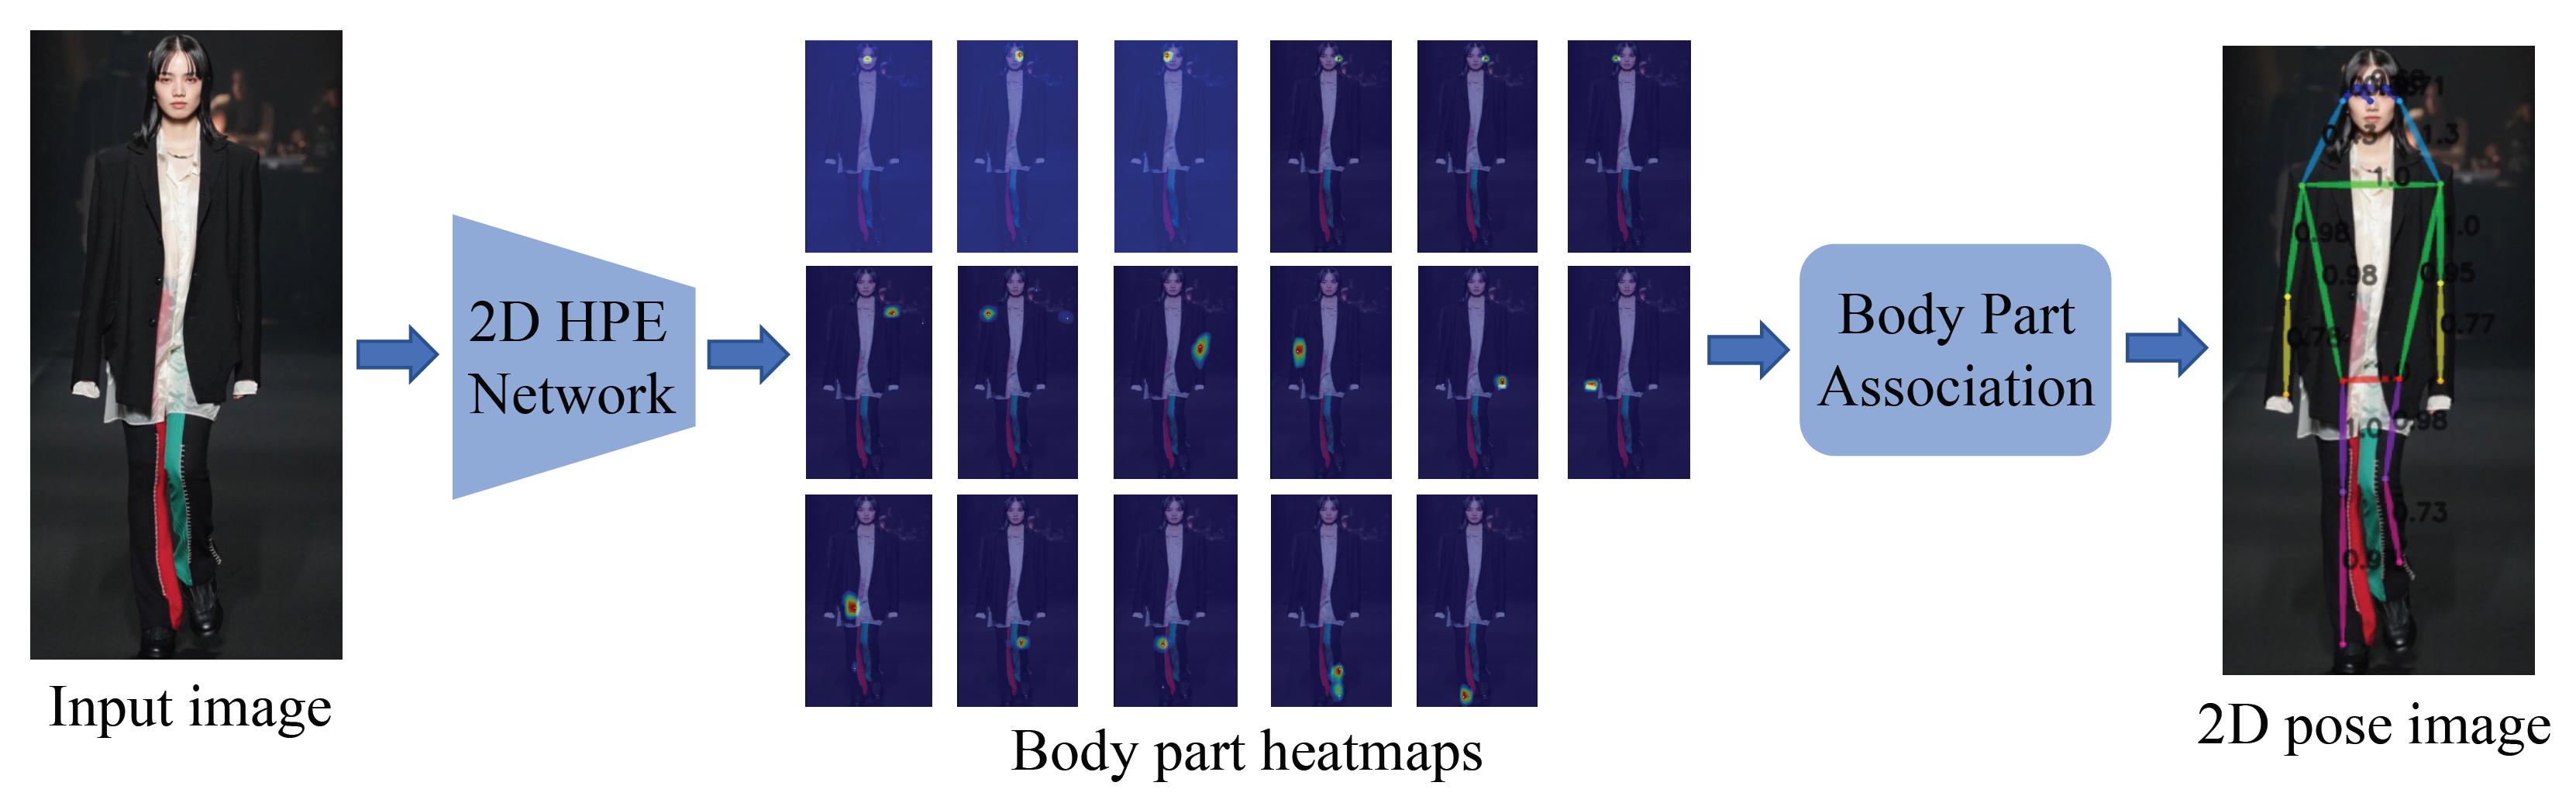
\includegraphics[width=0.8\textwidth]{single_pose_estimation_heatmap-based_methods}%
	\caption{Single-Person HPE Heatmap-based Methods as presented in \cite{Zheng2012}}
	\label{fig:single_pose_estimation_heatmap-based_methods}
\end{figure}

A fundamental work written by Wei et al. \cite{Wei2016} combines convolution networks with Pose Machines \cite{Ramakrishna2014}.
Pose Machines is an iterative architecture which consists of two models:
The first is used for stage one where it predicts potential heatmaps for the joints.
The second model is used for subsequent stages where the result of the previous stage is fed in together with the results of its own convolution network on the input image. 
This gradually refines the predictions for the joints and their positioning.
Another influential work was being written at the same time by Newell et al. \cite{Newell2016}.
Similar to \gls{CPMs}, this is also an iterative architecture.
They suggest what they call a "stacked hourglass" network, where "hourglass" modules are repeated.
In an "hourglass" module, first, the features are downsampled and, afterwards, upsampled again.
This network captures different spatial relationships between joints at different resolutions.
Several other works \cite{Yang2017, Chou17} have since improved on the network design.
Both use intermediate supervision to tackle the problem of vanishing gradients.
This still doesn't build a deep sub-network for feature extraction which limits the predictions.
This has become less of a problem with the emergence of the \gls{ResNet} \cite{He2015} which allows better back-propagation at deeper levels through shortcuts.

\begin{figure}[h]
	\centering
	\subcaptionbox{HRNet \label{fig:single_pose_estimation_HRNet}}[0.39\textwidth]{%
		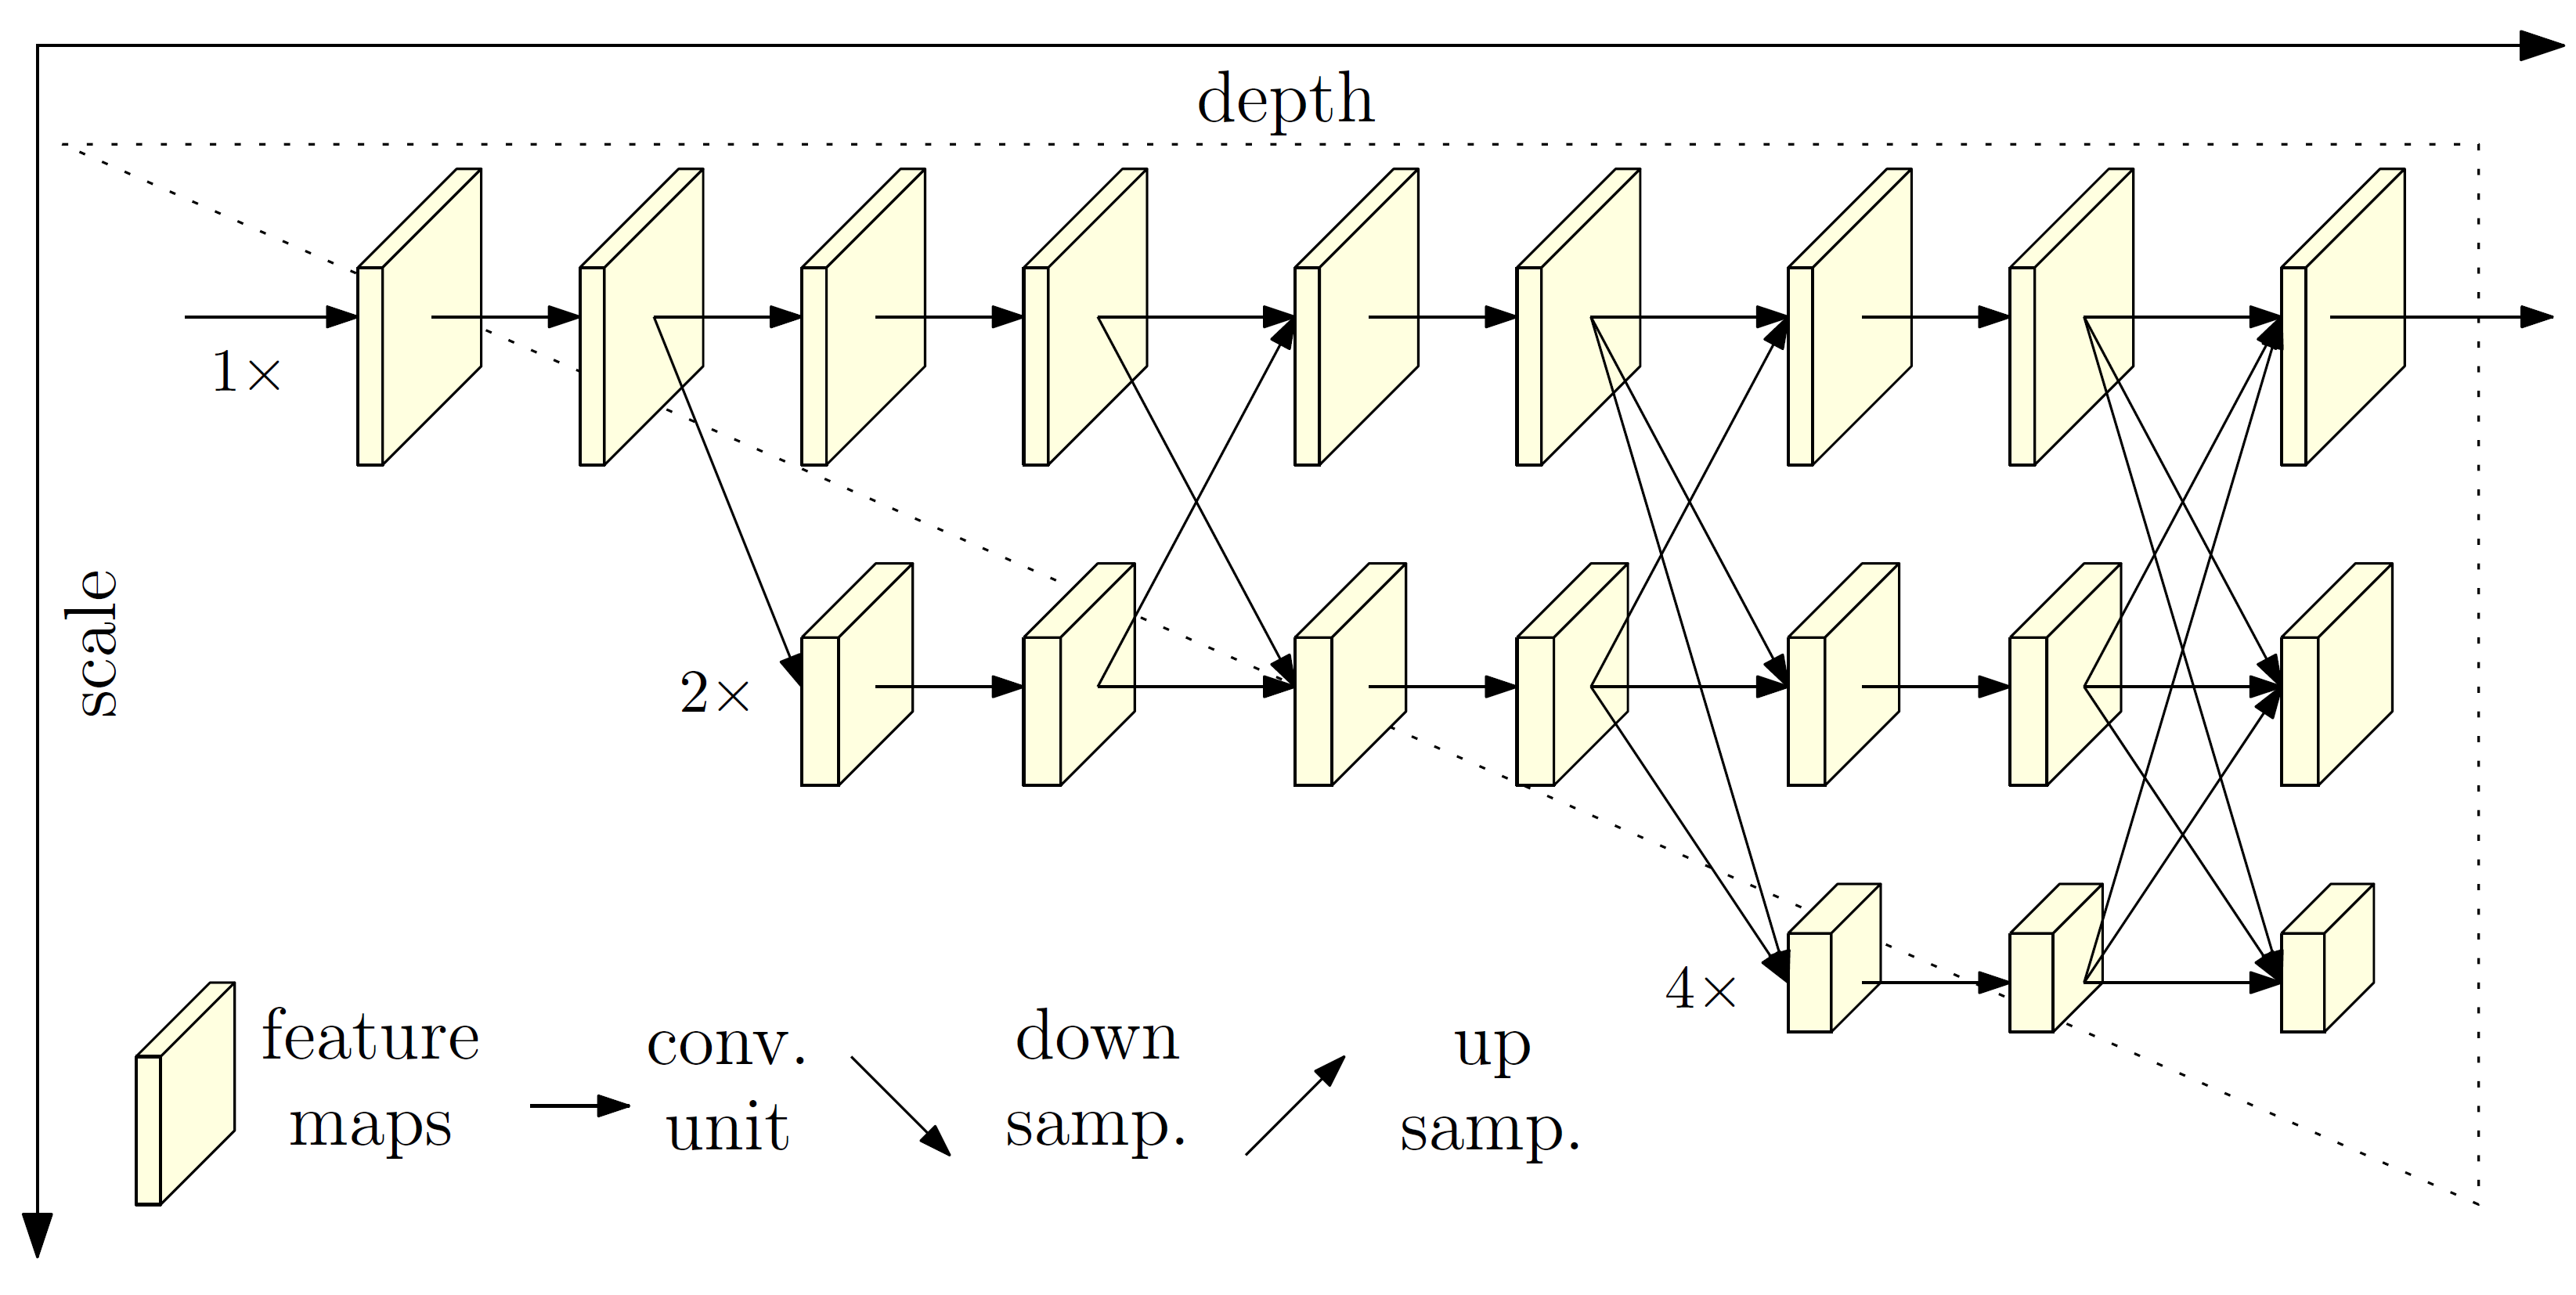
\includegraphics[width=0.39\textwidth]{single_pose_estimation_HRNet}%
	}
	\subcaptionbox{Multi-Scale Fusion \label{fig:single_pose_estimation_multi-scale_fusion}}[0.59\textwidth]{%
		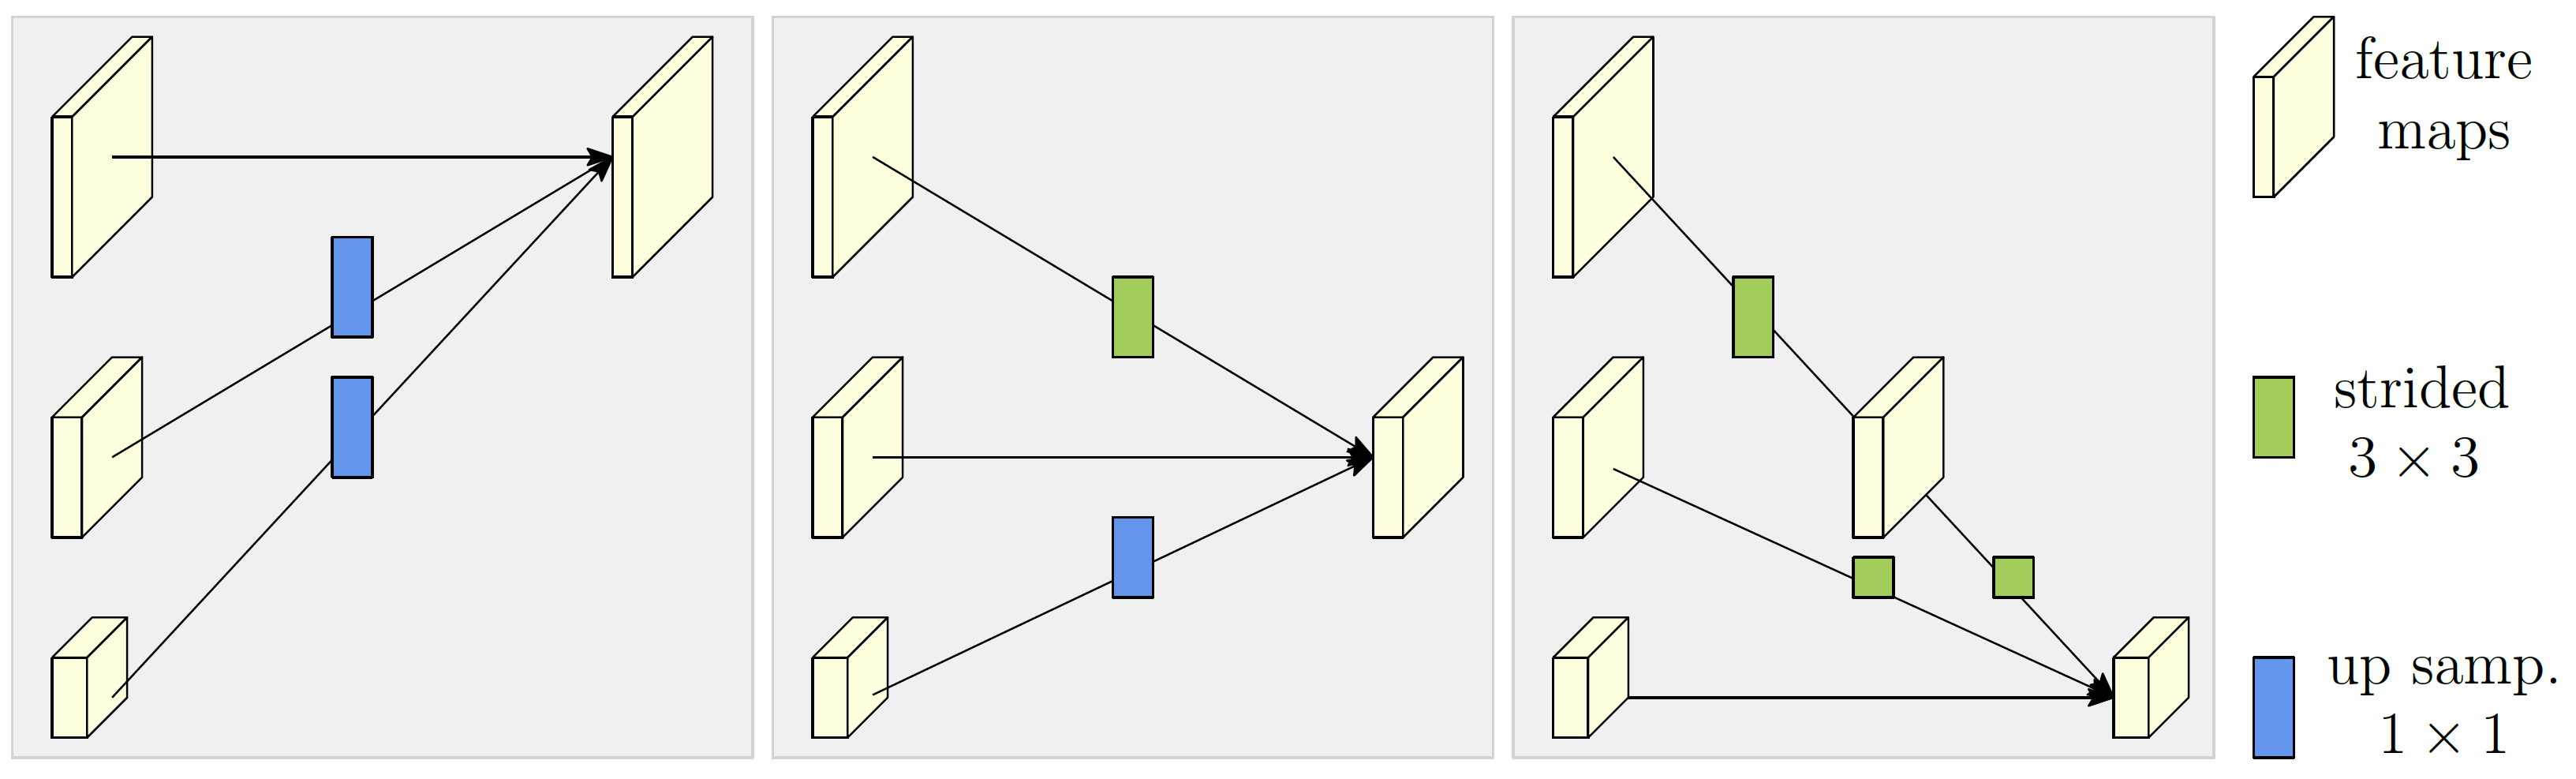
\includegraphics[width=0.59\textwidth]{single_pose_estimation_multi-scale_fusion}%
	}
	\caption{
		The architecture of the High-Resolution network and how it applies multi-scale fusion \cite{Sun2019}.
	}
	\label{fig:HRNet}
\end{figure}

A more recent work by Sun et al. \cite{Sun2019} maintains high-resolution representations instead of working with the high-resolution from the low-to-high sub-network.
After a first high-resolution sub-network, it gradually adds high-to-low sub-networks in parallel to predict multi-resolution features.
Before each branch, they apply multi-scale fusion, which joins the predicted features from each scale on each other scale (Figure \ref{fig:HRNet}).
This network has proven very effective and inspired several variations \cite{Cheng2019, Yu2021, Yuan2021}.
Chen et al. \cite{Chen2017b} propose using \gls{cGAN} \cite{Mirza2014} to improve constraints of joint inter-connectivity and infer occluded body parts.
A structure-aware convolution network using a stacked hourglass serves as generator which generates pose heatmaps as well as occlusion heatmaps for each joint.
Two discriminators are used, one to discriminate between low- and high-confidence predictions, another for real and fake poses.
A more classic GAN is used by Chou et al. \cite{Chou2017}, where they use a stacked hourglass network for both the generator as the discriminator.
The generator predicts the heatmaps for each joint and the discriminator distinguished between the real and fake ones.

\subsection{Multi-Person Methods}
With multi-person methods comes an extra layer of difficulty; they need to detect each person separately.
To solve this problem multi-person methods propose several solutions. 
The two most popular are top-down and bottom-up methods.

\textbf{Top-Down Methods} will first try to detect all persons in the image with a human detector.
Each person is cropped by the bounding box and a single-person estimator predicts a pose.
Occlusion and truncation are a regular occurrence in multi-person scenes and an inevitable problem.
One of the early multi-person models, by Iqbal et al. \cite{Iqbal2016}, creates a robust model against occlusion.
It uses \gls{Faster R-CNN} \cite{Ren2015} to detect the human boundaries, after which it applies integer linear programming on each person's fully connected graph to obtain the final pose estimates.
This technique is similar to \cite{Pishchulin2015}, but, instead of working on all globally found joints, it only considers local joints.
It can also handle any kind of occlusion or truncation.
The use of a human detector comes with its own set of problems, which Fang et al. \cite{Fang2016} try to remedy with \gls{RPME}.
Their solution consists of two components:
They try to tackle inaccurate bounding boxes with a Symmetric Spatial Transformer Network and redundant detections with Parametric Pose Non-Maximum-Suppresion.
They also propose a 3rd component, the Pose-Guided Proposals Generator, which can augment training samples.
Papandreou et al. \cite{Papandreou2017} use a two stage pipeline.
In the first stage, they employ the Faster R-CNN detector.
In the second stage, they estimate the pose in each found bounding box using their own network.
It predicts heatmaps using a fully convolutional \gls{ResNet} and then uses their own novel aggregation procedure.
Afterwards, they do post-processing using keypoint-based \gls{NMS}; a method of their own making.
A continuous effort is taken by Chen et al. \cite{Chen2017a} to deal with occlusion and truncation.
They suggest a two stage architecture, where first the "simple" keypoints are captured with GlobalNet, a feature pyramid network based on \cite{Lin2016}, and the "hard" keypoints are handled by their RefineNet.
It integrates the information via upsampling and concatenating of HyperNet \cite{Kong2016} and using an adapted stacked hourglass.
They achieved great results and several others improved on their work \cite{Su2019, Li2019a}.
In more recent research, a new method was become competitive with \glspl{CNN}.
Based on work in language modeling, attention mechanisms, an optimization of recurrent networks, allow the modeling of dependencies without regard of the distance in the input or output sequences.
The Transformer, introduced by Vaswani et al. \cite{Vaswani2017}, eliminates recurrence and relies solely on attention mechanisms.
This enables it to work better in parallel while it still maintains state-of-the-art performance.
Based on this new architecture, Dosovitskiy et al. \cite{Dosovitskiy2020} created a new model that can work with images; the \gls{ViT}.
Xu et al. \cite{xu2022} use the vision transformer to apply it to the HPE task.
As seen in Figure \ref{fig:vitpose}, they try to keep the network simple and don't use certain optimizations that can increase complexity.
It works by splitting the input image into fixed-size patches which are linearly embedded and then fed into the transformer blocks.
The output of this is then processed by different decoders to form the heatmaps.
To show the strong representation ability of transformers the authors provide a simple decoder next to the classic decoder and show that even the simple decoder obtains competitive results.

\begin{figure}[h]
	\centering
	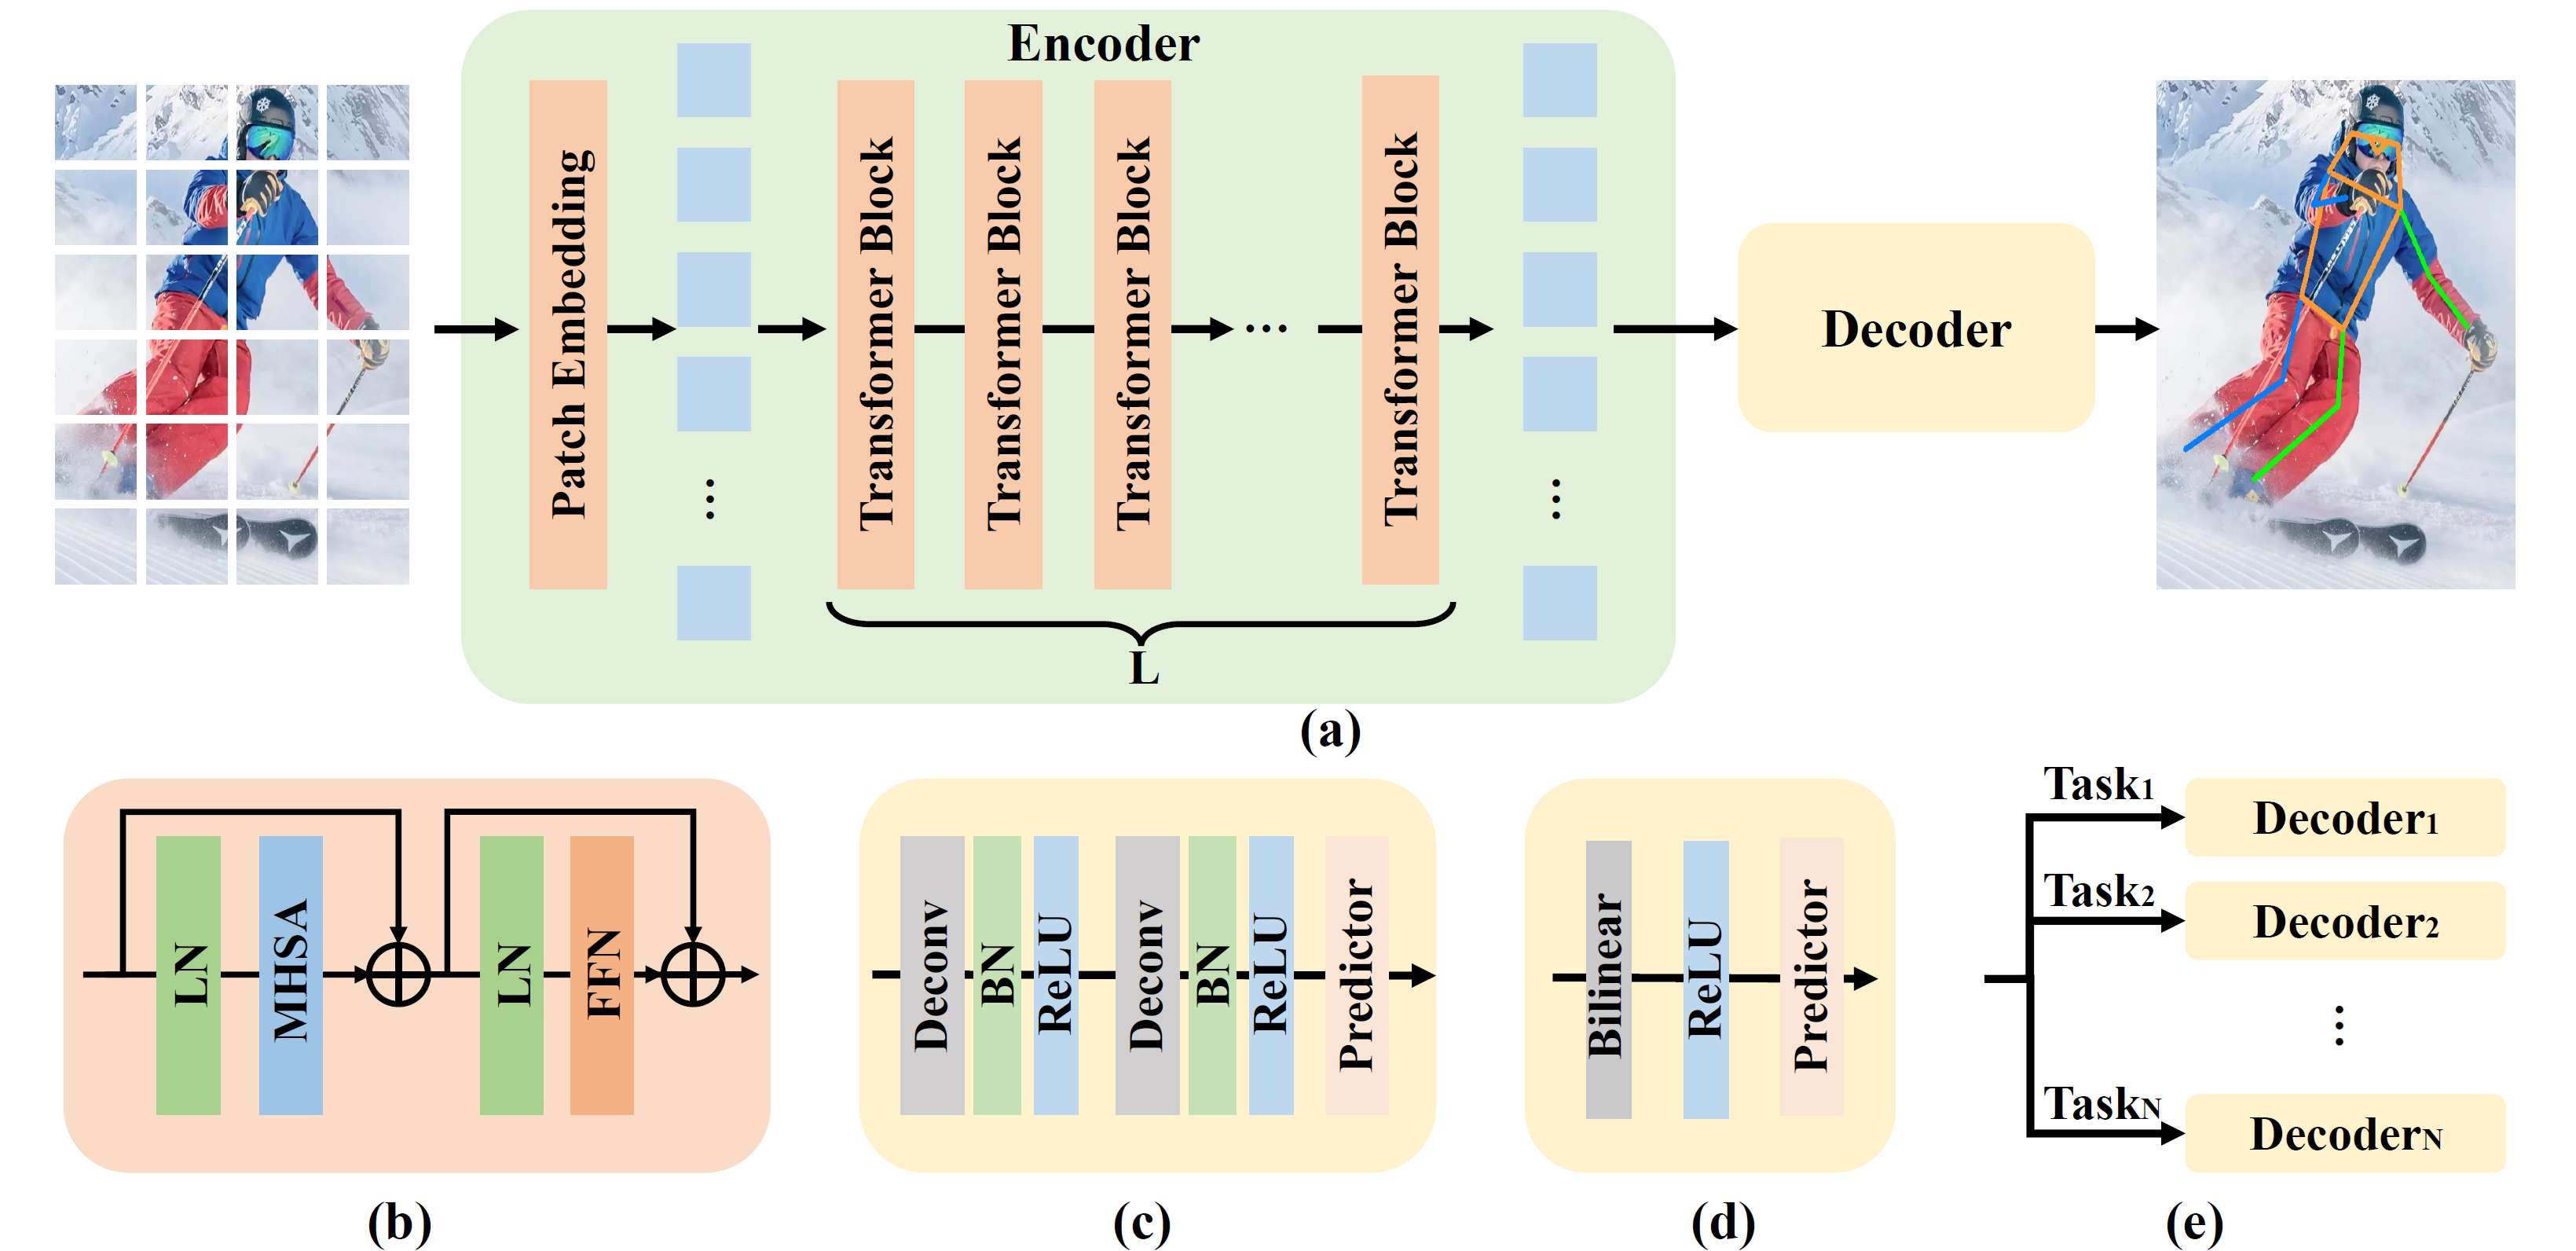
\includegraphics[width=0.8\textwidth]{vitpose}%
	\caption{
		(a) The framework of ViTPose. (b) The transformer block. (c) The classic decoder. (d) The simple decoder. (e) The decoders for multiple datasets. \cite{xu2022}
	}
	\label{fig:vitpose}
\end{figure}

\textbf{Bottom-Up Methods} use a different approach to predict the keypoints.
They first locate all joints in the image and then afterwards assemble them in potential poses.
DeepCut by Pishchulin et al. \cite{Pishchulin2015} is one of the first multi-person models using \glspl{CNN}.
Using Fast R-CNN \cite{Ren2015}, it detects the body parts and labels each.
With the joints found, it then uses \gls{ILP} to assemble them.
However, this method is very computationally expensive; NP-hard.
Insafutdinov et al. \cite{Insafutdinov2016} therefor introduce a stronger part detector and better optimization strategy with DeeperCut.
\gls{CPMs} make a return with OpenPose by Cao et al. \cite{Cao2018}.
They're used to predict the joints with heatmaps and \glspl{PAFs}.
PAFs also encodes the position and orientation of the limb which makes the assembly of joints into different poses more reliable.
They can achieve real-time results with this method, and several others have improved on their design \cite{Zhu2017a, Hidalgo2019, Li2019b}.
The high performance is only applicable to high-resolution images and low-resolution images or images with occlusions perform poorly.
Kreiss et al. \cite{Kreiss2019} continue on the idea of fields and introduce the \gls{PIF} and \gls{PAF}.
First, they predict the location of the different joints with \gls{PIF}.
Afterwards, they use \gls{PAF} to find the inter-joint relationships.
They are able to outperform any previous OpenPose-based proposals on low-resolution and occlusions.
Newell et al. \cite{Newell2016-2} introduce associative embedding which is a new method to represent the output.
This is a single-stage architecture as opposed to the two-staged architectures previously discussed.
They make use of the stacked hourglass network from \cite{Newell2016} with some small modifications, and produce joint heatmaps and associative embedding tags.
Continuing on the idea of associative embedding, Cheng et al. \cite{Cheng2019} use HRNet \cite{Sun2019} as backbone for their HigherHRNet (Figure \ref{fig:higherhrnet}).
Their method focuses on the scale-variance problem; a problem which hasn't been studied much, so it can localize keypoints for small persons better.
Lou et al. \cite{Lou2020} introduce \gls{SAHR} and \gls{WAHR} to the scale-variance problem.
\gls{SAHR} adaptively adjusts the standard deviation of each heatmap corresponding with the scale of the person.
\gls{WAHR} rebalances the foreground and background samples, so \gls{SAHR} can work to its fullest extent.

\begin{figure}[h]
	\centering
	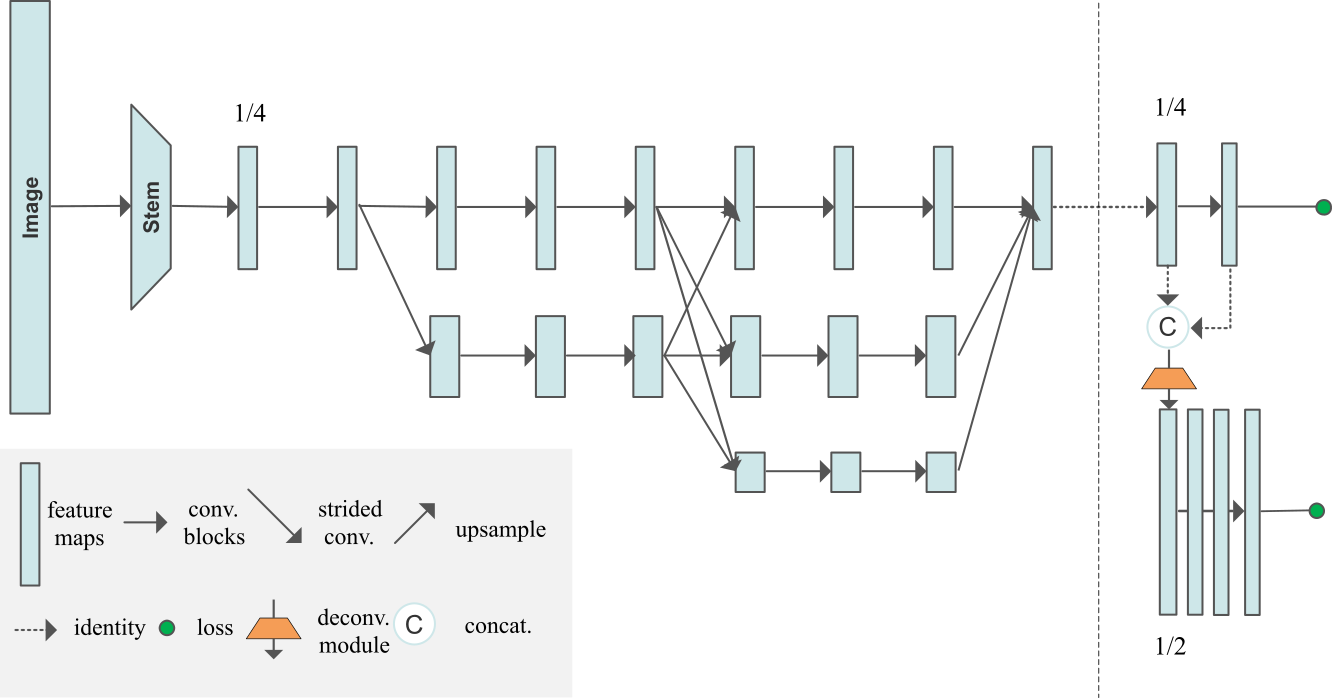
\includegraphics[width=0.5\textwidth]{higherhrnet}%
	\caption{
		The architecture of HigherHRNet. It uses HRNet as backbone. \cite{Cheng2019}
	}
	\label{fig:higherhrnet}
\end{figure}

\subsubsection{Summary}
An important challenge for HPE is making predictions in scenes with hight occlusions.
Top-down models achieve state-of-the art performance on almost all benchmark datasets \cite{Chen2000}.
However, they have difficulty with overlapping bodies and human detectors add an extra layer of failure.
To the same extent, bottom-up models have greater inaccuracy when grouping in occluded scenes.
Computationally, the top-down model's speed is heavily bound to the number of people the human detector finds.
The higher efficiency of bottom-up models make them more suitable for real-time applications.

\subsection{Evaluation Metric}
The evaluation of an HPE looks to measure the accuracy of the location of predicted joints.
Because of the different number of features and tasks across datasets, there are also several different evaluation metrics in use.
Explained next will be the most commonly used metrics.

\begin{enumerate}
	\item \textbf{Percentage of Correct Parts (PCP)}, proposed by Ferrari at al. \cite{Ferrari2008}, measures the detection rate of limbs.
	A limb is considered the area between two joints and viewed as detected when the distance between the predicted joints and the real joints is less than halve the length of the limb.
	This method penalizes shorter limbs and to address this, \gls{PDJ} was introduced which instead measures it with a fraction of the torso diameter.
	The higher, the better.
	\item \textbf{Percentage of Correct Keypoints (PCK)}, suggested by Yang et al. \cite{Yang2013}, measures the accuracy of the predicted keypoints.
	The keypoints should be within a certain threshold, which is a fraction of the person's bounding box size; denoted as PCK@0.2 when it should be less than 20\%.
	It can also be 50\% of the head's length; denoted as PCKh@0.5, which makes it "articulation independent".
	The higher, the better.
	\item \textbf{Average Precision/Recall (AP/AR)}, by Yang et al. \cite{Yang2013}, is calculated by counting a keypoint that is within a certain threshold of the ground truth as a true positive.
	For Lin et al. \cite{Lin2014}, the AP is calculated by measuring the \gls{OKS} (Figure \ref{fig:keypoint-similarity-distribution}) which is similar to Intersection over Union in Object Detection.
	The \gls{OKS} is defined as:
	\begin{equation}
		\operatorname{OKS} = \frac{\sum_{i}\exp(-d_i^2/2s^2k_i^2)\delta(v_i > 0)}{\sum_i \delta(v_i > 0)}
	\end{equation}
	Here, $d_i$ is the distance between the predicted keypoint and the ground truth.
	The distance is run through a unnormalized Gaussian with a standard deviation of $sk_i$ which yields a similarity that ranges between 0 and 1.
	$s$ is the scale, calculated as the root of the segment area, and $k_i$ is a constant for each keypoint that controls falloff.
	\gls{OKS} is the mean of visible keypoints ($v_i > 0$).
	These can be used to calculate \gls{AP} and \gls{AR} at different thresholds.
	10 different metrics are used to calculate the performance of a model:
	$\operatorname{AP}^{0.5}$ (where the $\operatorname{OKS}$ threshold is $0.5$), $\operatorname{AP}^{0.75}$ and $\operatorname{AP}$ (the mean of 10 values from $\operatorname{OKS}=0.50$ to $0.95$ with a $0.05$ step), as well as, $\operatorname{AP}^{M}$ for medium scaled objects and $\operatorname{AP}^{L}$ for large scaled objects.
	The same metrics are calculated for \gls{AR}.
	The higher, the better.
\end{enumerate}

\begin{figure}[h]
	\centering
	\captionbox{
		\label{fig:keypoint-similarity-distribution}
		An illustration of keypoint similarity.
		The predicted values (red and green) are at the same distance from the ground-truth (blue).
		The wrist and eye have a different $k_i$ causing a different falloff \cite{Ronchi2017}.
	}[0.86\textwidth]{
		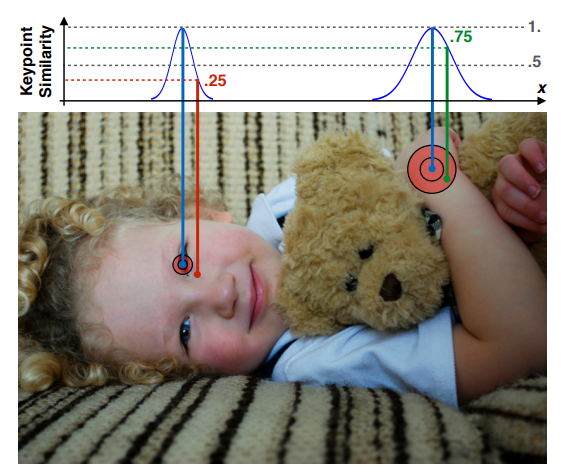
\includegraphics[width=0.5\textwidth]{keypoint-similarity-distribution}%
	}
\end{figure}

\section{Image Style Transfer}
Image Style Transfer is the technique of applying the style of one image to the content of another.
Traditionally, this is a problem reserved for only artists, but more recently this has also interested computer scientists.
There are several different ideas on how this can be achieved,
ranging from how to separate the style from the content to how well an algorithm can generalize.
An overview of all the different challenges and solutions will be given in this chapter.

\subsection{Datasets}
Due to a lack of benchmark datasets, multiple papers will mix and match from different datasets, like \gls{COCO} or ImageNet \cite{Deng2009}.

\begin{enumerate}
	\item \textbf{Cityscape Dataset \cite{Cordts2016}} consists of 2975 images of cityscapes with semantic annotations.
	\item \textbf{Facades Dataset \cite{Tylecek2013}} consists of 400 images of building facades with architectural annotations.
	\item \textbf{Maps Dataset \cite{Isola2016}} consists of 1096 images of maps and areal photos gathered from Google Maps around New York City.
	\item \textbf{Edges2shoes Dataset \cite{Yu2014}} consists of 50,000 paired images between edges and photos of shoes.
	\item \textbf{Edges2handbags Dataset \cite{Zhu2016}} consists of 137,000 paired images between edges and photos of handbags.
	\item \textbf{Horse $\leftrightarrow$ Zebra \cite{Zhu2017b}} consists of 2,500 images of 512x512 horses and zebras, that were sampled from ImageNet \cite{Deng2009}.
	\item \textbf{Animal Face High Quality \cite{Choi2019}} consists of 15,000 high quality images of 512x512 animal faces, including cat, dog and wildlife.
	\item \textbf{Night2Day Dataset \cite{Laffont2014}} consists of 20,000 images taken from time-lapse datasets and annotated through crowdsourcing.
	\item \textbf{WikiArt Dataset \cite{Saleh2015}} consists of 80,000 fine-art paintings.
	All are annotated for 27 styles, 60,000 are annotated for 20 genres and 20,000 for 23 artists.
\end{enumerate}

\subsection{Optimization-based Networks}
Gatys et al. \cite{Gatys2016} introduce deep neural networks to image style transfer.
As seen in Figure \ref{fig:style_transfer_algorithm}, using a modified VGG-network \cite{Simonyan2015}, they extract the features from the higher layers of an image, which they argue represents the content, and then reconstruct it on a white noise image.
They also extract the style representation of another image by using the Gram matrix and then reconstructs it on the same white noise image.
The Gram matrix is the vector product of two sets of vectorized feature maps.
They remark that the resolution affects the performance of the algorithm and is thus restricted to low resolutions.
At the same time, the synthesized images contain some low-level noise, but this can be removed with a denoiser.

\begin{figure}[h]
	\centering
	\captionsetup{justification=centering}
	\captionbox{
		\label{fig:style_transfer_algorithm}
		Style transfer algorithm by Gatys et al. \cite{Gatys2016}. \\
		The left side transfers the style from a given image, the right side the content.
	}[0.86\textwidth]{
		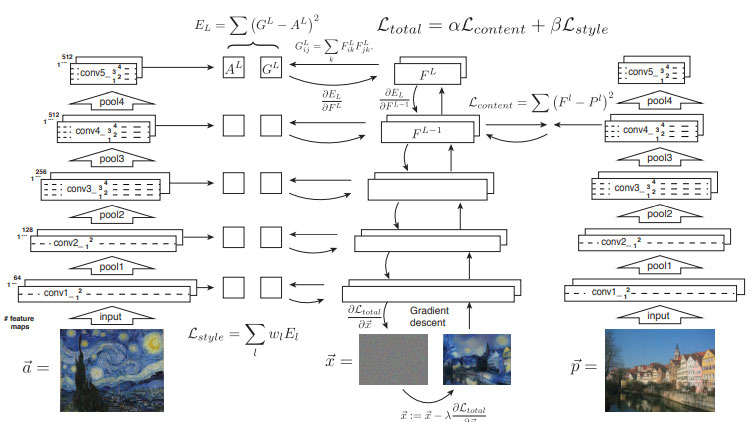
\includegraphics[width=0.7\textwidth]{style_transfer_algorithm}
	}
\end{figure}

\subsection{Feed-forward Generation Networks}
To improve the performance, Ulyanov et al. \cite{Ulyanov2016} suggest using a feed-forward generation network instead of reconstruction.
Reconstruction requires an iterative process to change the pixel values to match the desired statistics.
A feed-forward network can do this in a single evaluation.
To train such a network, they use a pre-trained network for image classification, and calculate a texture and content loss by extracting the features similar to \cite{Gatys2016}.
Johnson et al. \cite{Johnson2016} propose an almost identical framework independently.
The work of Ulyanov et al. did increase the performance, but at the expense of quality, therefor they suggest further improvements to their network \cite{Ulyanov2017}.
First, they replace \gls{BN} \cite{Ioffe2015} with \gls{IN} which alone has a significant impact on quality as can be seen in \ref{fig:style_transfer_ulyanov_BN_IN_comparison}.
Second, they teach the generator to sample from the Julesz ensemble \cite{Zhu2000} which improves variation in the outputs.
\\

\begin{figure}[h]
	\centering
	\subcaptionbox{Content Image \label{fig:style_transfer_ulyanov_content}}[0.18\textwidth]{%
		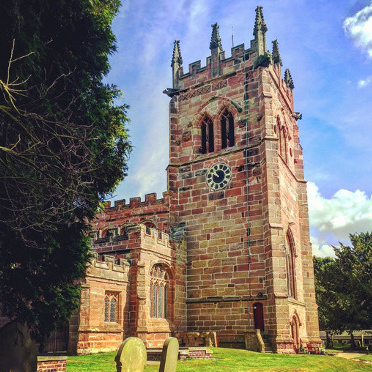
\includegraphics[width=0.18\textwidth]{style_transfer_ulyanov_content_2}\\
		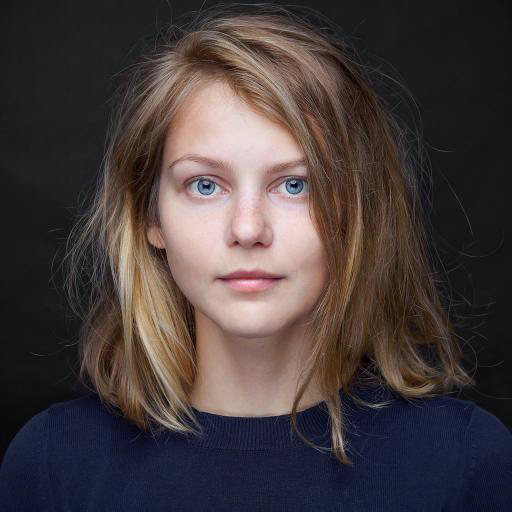
\includegraphics[width=0.18\textwidth]{style_transfer_ulyanov_content}%
	}
	\subcaptionbox{Style Image \label{fig:style_transfer_ulyanov_style}}[0.18\textwidth]{%
		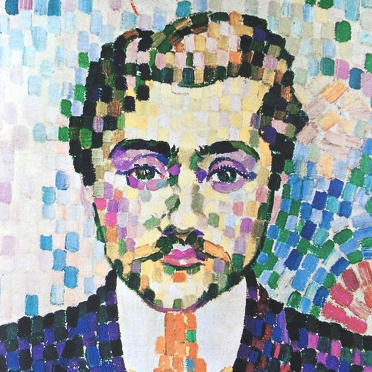
\includegraphics[width=0.18\textwidth]{style_transfer_ulyanov_style_2}\\
		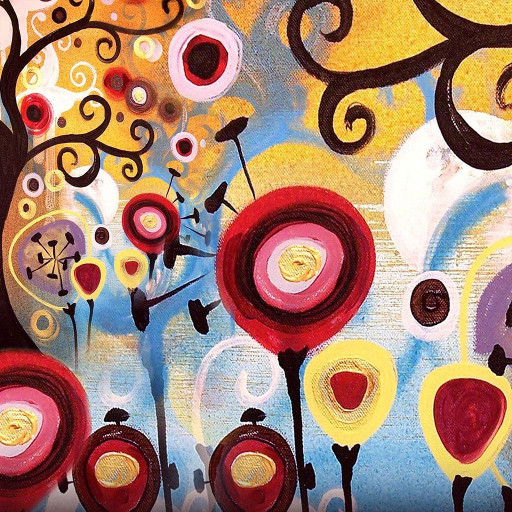
\includegraphics[width=0.18\textwidth]{style_transfer_ulyanov_style}%
	}
	\subcaptionbox{StyleNet with BN \label{fig:style_transfer_ulyanov_BN}}[0.18\textwidth]{%
		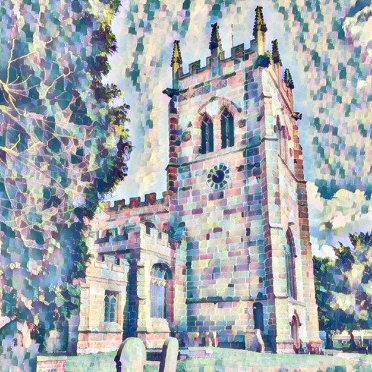
\includegraphics[width=0.18\textwidth]{style_transfer_ulyanov_BN_2}\\
		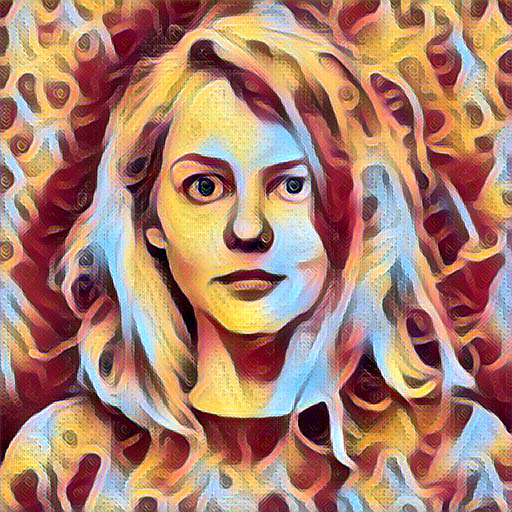
\includegraphics[width=0.18\textwidth]{style_transfer_ulyanov_BN}%
	}
	\subcaptionbox{StyleNet with IN \label{fig:style_transfer_ulyanov_IN}}[0.18\textwidth]{%
		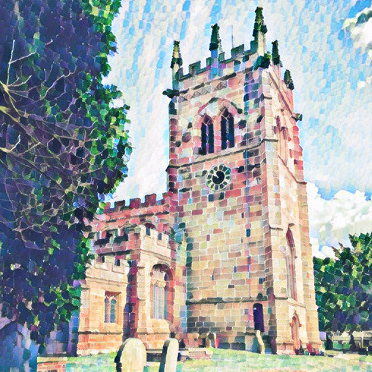
\includegraphics[width=0.18\textwidth]{style_transfer_ulyanov_IN_2}\\
		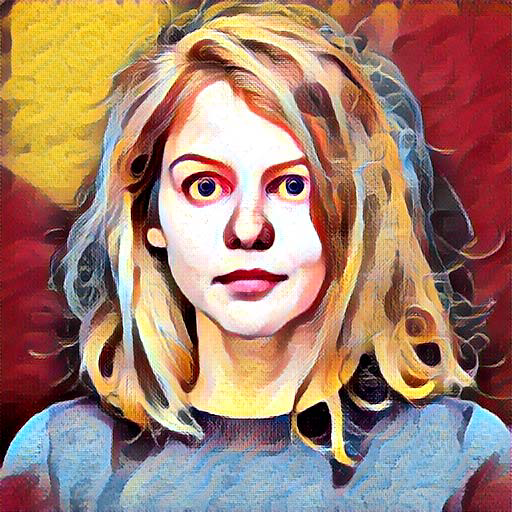
\includegraphics[width=0.18\textwidth]{style_transfer_ulyanov_IN}%
	}
	\caption{A comparison between (c) BN and (d) IN.\cite{Ulyanov2017}}
	\label{fig:style_transfer_ulyanov_BN_IN_comparison}
\end{figure}

Dumoulin et al. \cite{Dumoulin2016} observe that previous feed-forward networks are limited to one style.
In order to facilitate many different styles, there would need to be a network trained separately for each which limits the applications for mobile devices.
In order to make the network more memory efficient, they propose a conditional style transfer network; given a content image and a style name, it transforms the image to the corresponding style.
They argue that after normalization each style can be distinguished by specializing scaling and shifting parameters.
They call this \gls{CIN}.
Since it only changes the scale and shift parameters for different styles, the network requires fewer parameters.
Of the 1.6M parameters, only 3K are needed for the different styles.
Another network that puts a focus on multiple styles comes from Chen et al. \cite{Chen2017c}.
They propose a StyleBank which can store multiple convolution filter banks each representing a different style.
They use an autoencoder with in between the encoder and decoder a StyleBank layer.
During training, for each $T+1$ iterations the entire network is first trained with a perception loss for the first $T$ iterations.
Then only the autoencoder network is trained with a \gls{MSE} loss.
This way the autoencoder only retains the content and the StyleBank layer only the different styles.
This also allows them to lock the encoder and decoder to learn a new style afterwards.
While \gls{CIN} allows for multiple styles, it's still limited to the ones that were seen during training.
Huang et al. \cite{Huang2017} try to remedy this by introducing an \gls{AdaIN} layer.
Unlike the other normalization techniques, \gls{AdaIN} does not have affine parameters, and will adaptively compute these from the style image.
Figure \ref{fig:adaptive_instance_normalization} shows that their network first extracts features from the content and style image using a fixed VGG-19 network as their encoder.
The AdaIN layer then performs style transfer in the feature space and with the results the decoder constructs a new image.
During training, the content loss and style loss are calculated by extracting the features using the same VGG encoder.
To make a comparison between different networks and how they deal with unseen styles, Figure \ref{fig:style_transfer_unseen_style} gives an overview.

\begin{figure}[h]
	\centering
	\captionsetup{justification=centering}
	\captionbox{
		\label{fig:adaptive_instance_normalization}
		Adaptive Instance Normalization network by Huang et al. \cite{Huang2017}. \\
	}{
		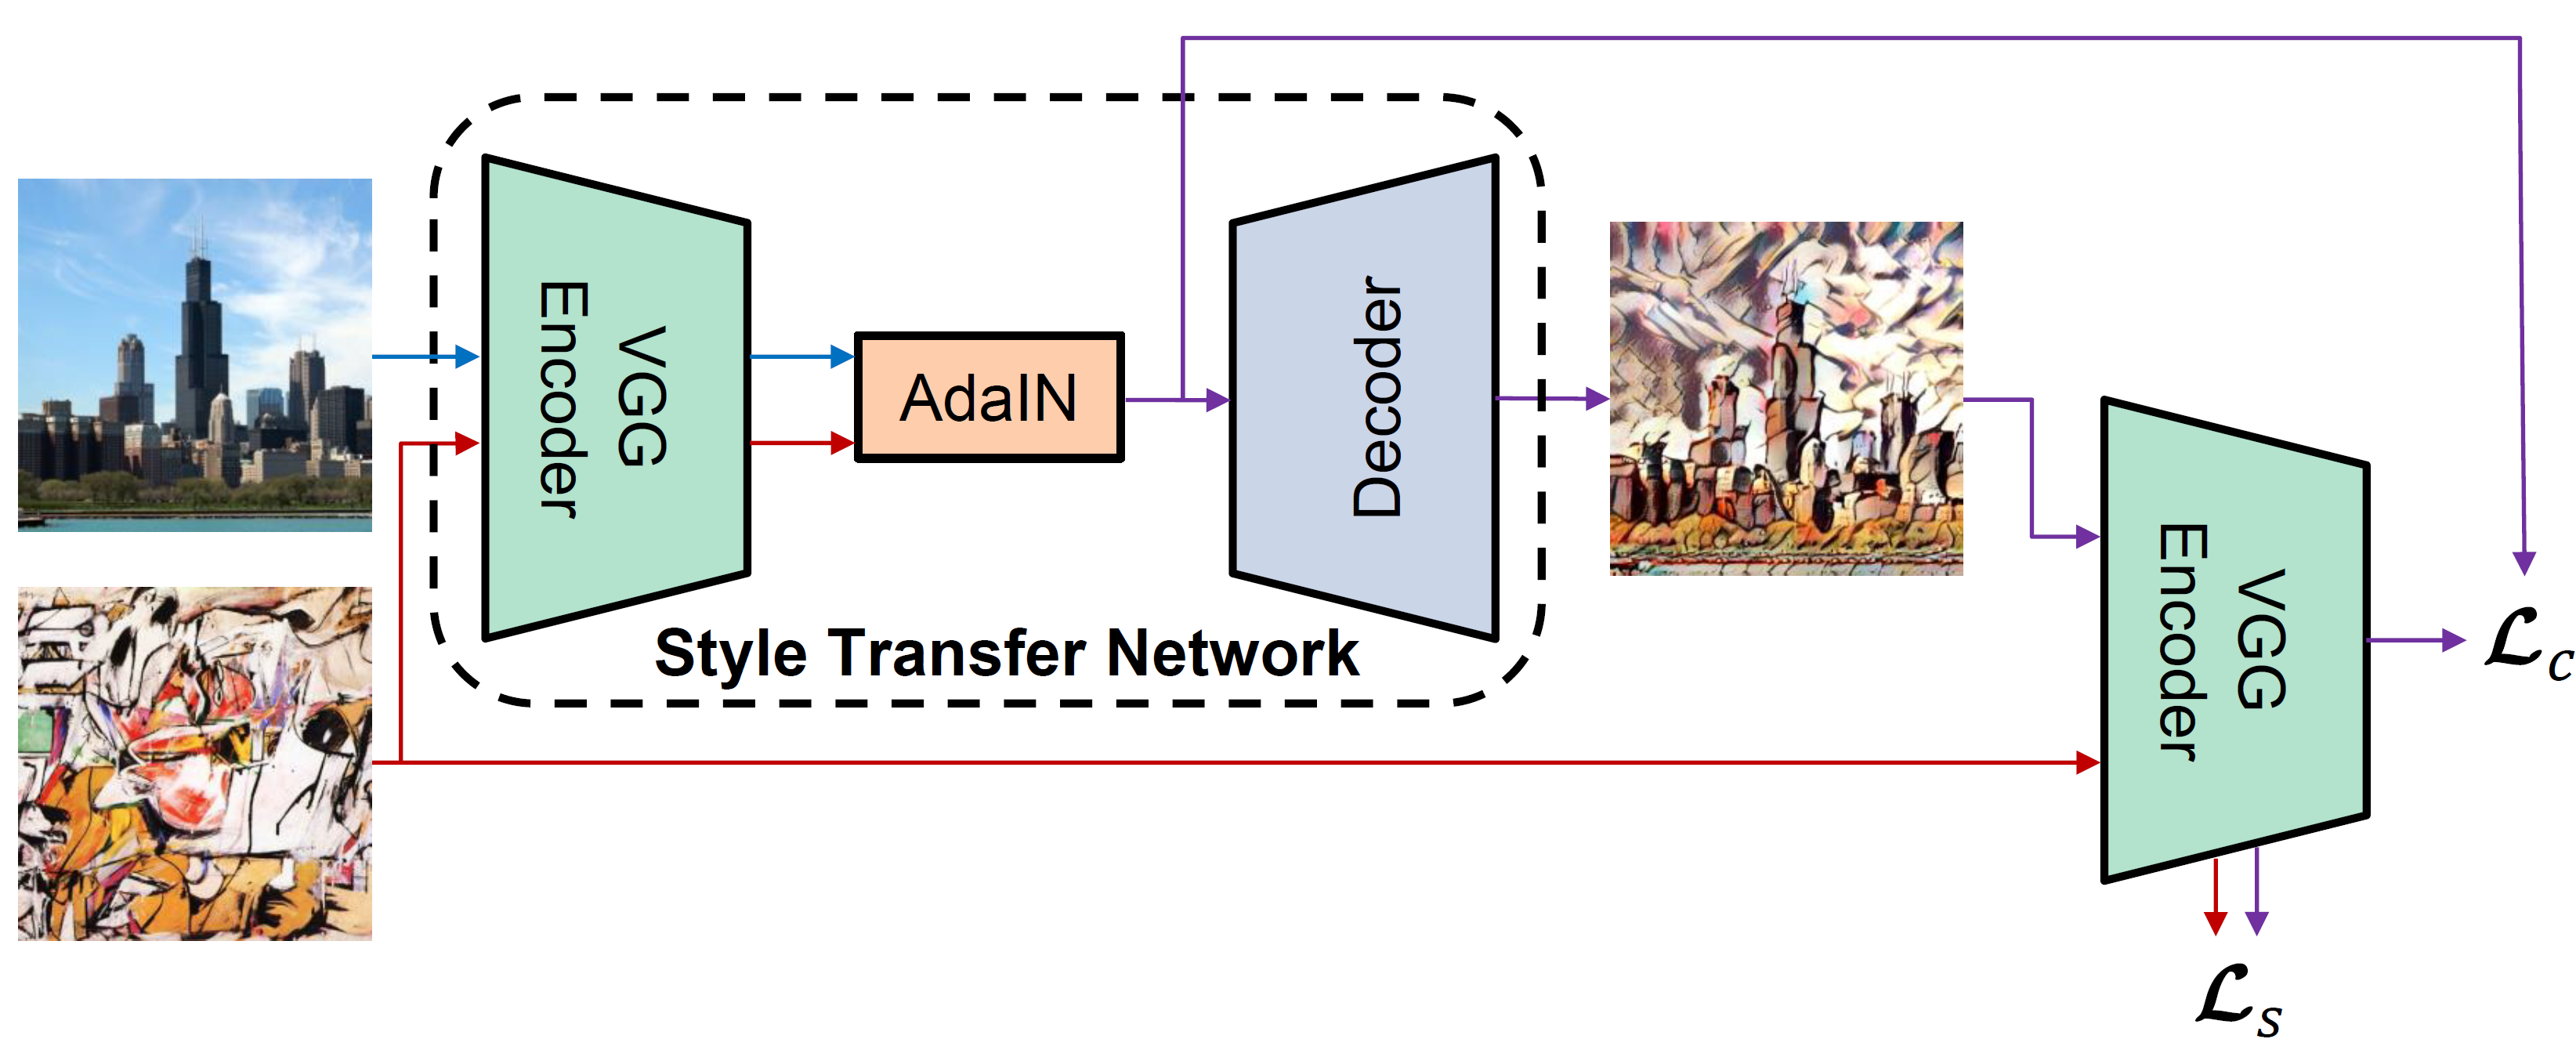
\includegraphics[width=0.8\textwidth]{adaptive_instance_normalization}
	}
\end{figure}

\begin{figure}
	\centering
	\subcaptionbox{Content Image}[0.19\textwidth]{
		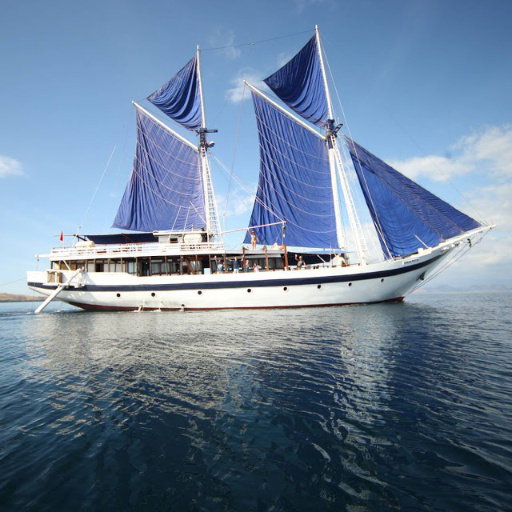
\includegraphics[width=0.19\textwidth]{style_transfer_content_a}\\
		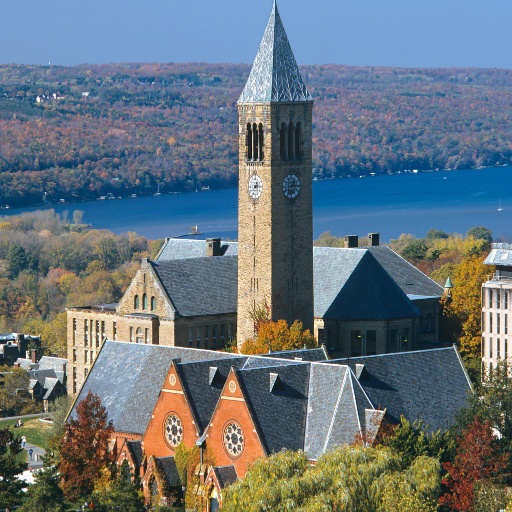
\includegraphics[width=0.19\textwidth]{style_transfer_content_b}\\
		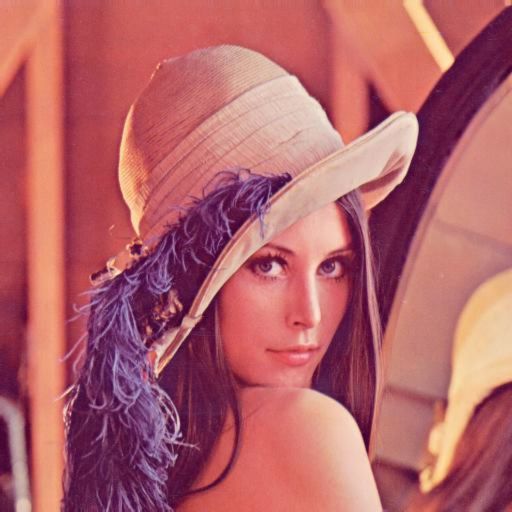
\includegraphics[width=0.19\textwidth]{style_transfer_content_c}\\
		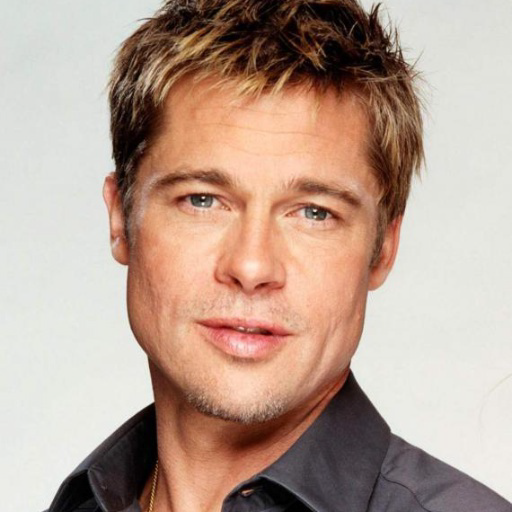
\includegraphics[width=0.19\textwidth]{style_transfer_content_d}\\
		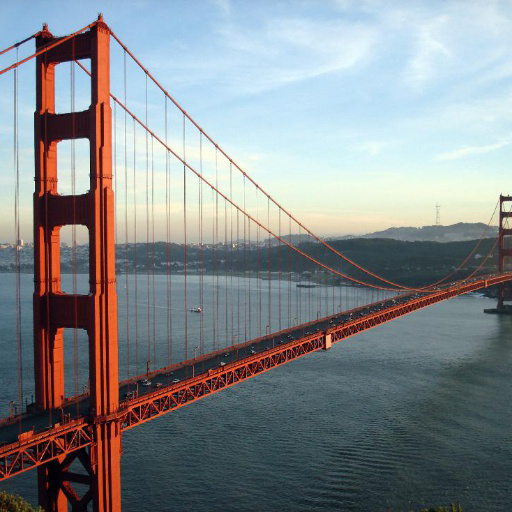
\includegraphics[width=0.19\textwidth]{style_transfer_content_e}\\
	}
	\subcaptionbox{Style Image}[0.19\textwidth]{
		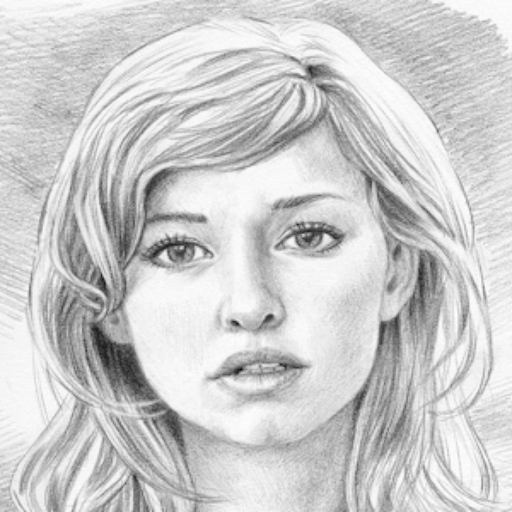
\includegraphics[width=0.19\textwidth]{style_transfer_style_a}\\
		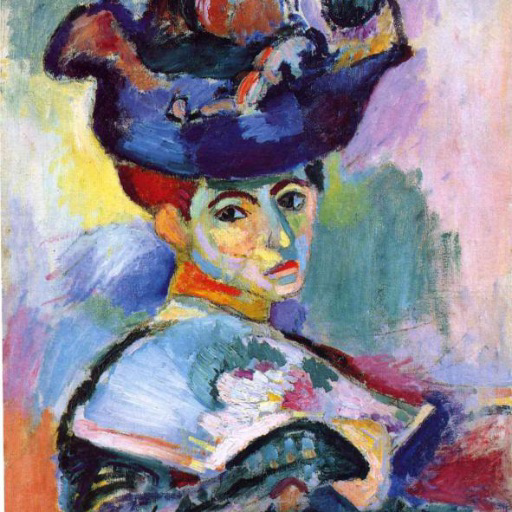
\includegraphics[width=0.19\textwidth]{style_transfer_style_b}\\
		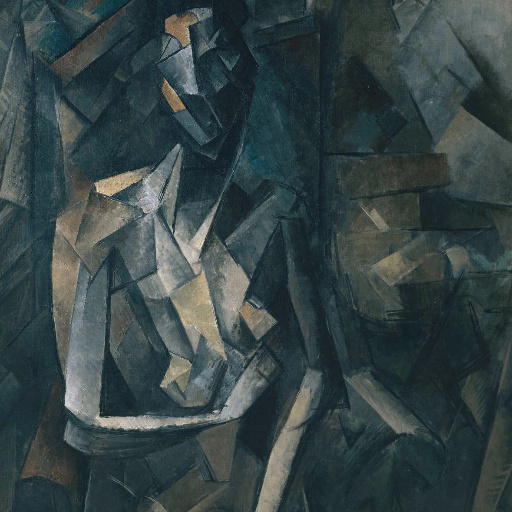
\includegraphics[width=0.19\textwidth]{style_transfer_style_c}\\
		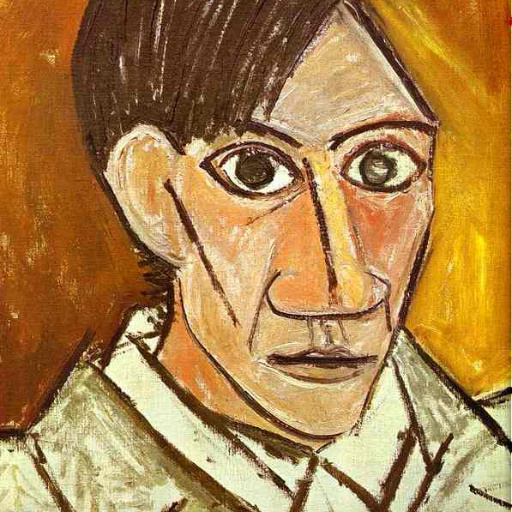
\includegraphics[width=0.19\textwidth]{style_transfer_style_d}\\
		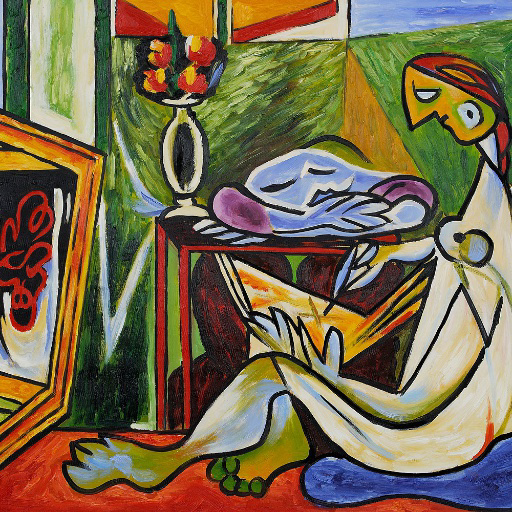
\includegraphics[width=0.19\textwidth]{style_transfer_style_e}\\
	}
	\subcaptionbox{Huang et al.}[0.19\textwidth]{
		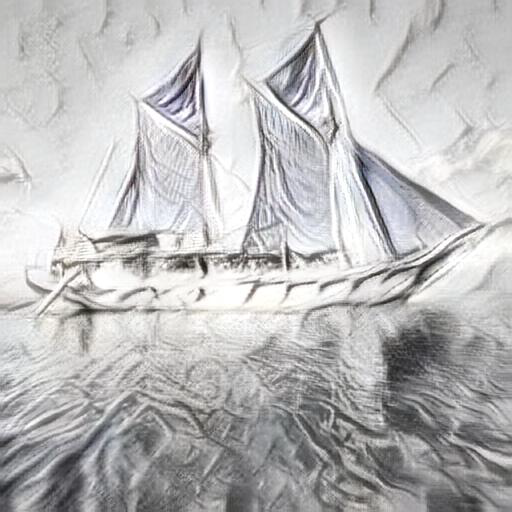
\includegraphics[width=0.19\textwidth]{style_transfer_huang_a}\\
		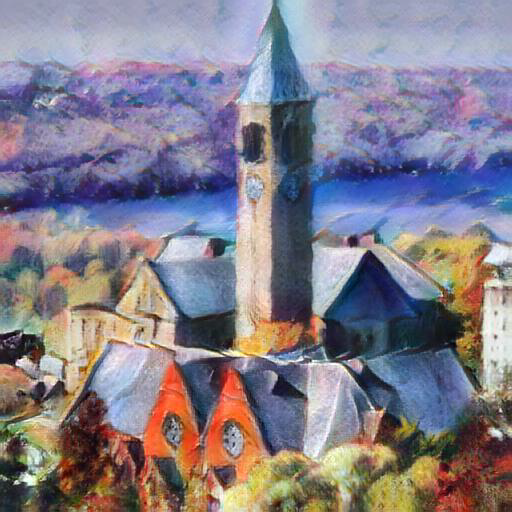
\includegraphics[width=0.19\textwidth]{style_transfer_huang_b}\\
		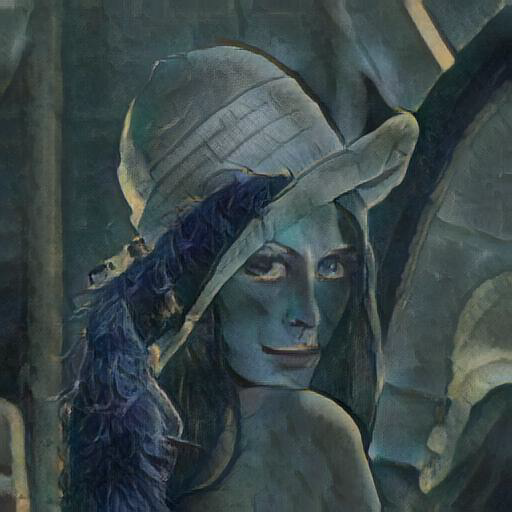
\includegraphics[width=0.19\textwidth]{style_transfer_huang_c}\\
		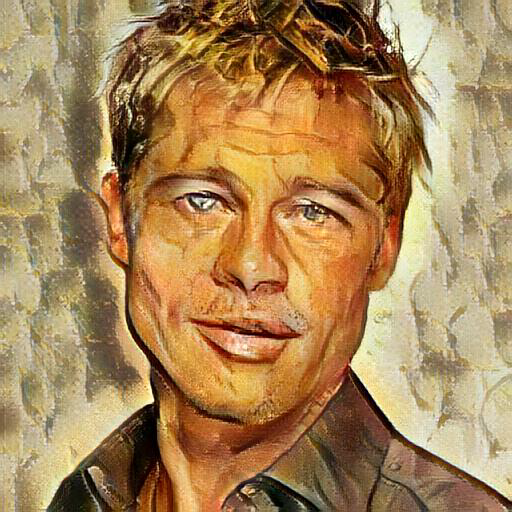
\includegraphics[width=0.19\textwidth]{style_transfer_huang_d}\\
		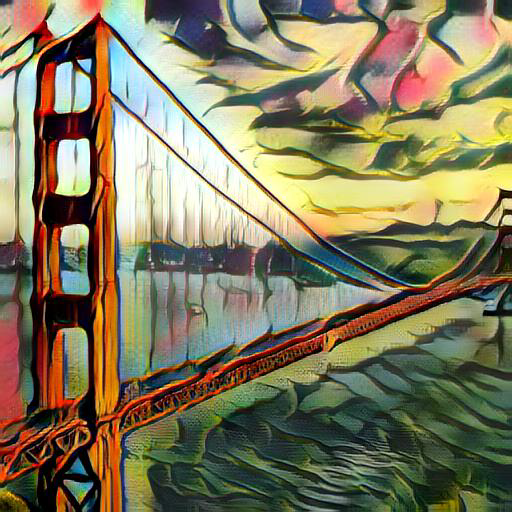
\includegraphics[width=0.19\textwidth]{style_transfer_huang_e}\\
	}
	\subcaptionbox{Ulyanov et al.}[0.19\textwidth]{
		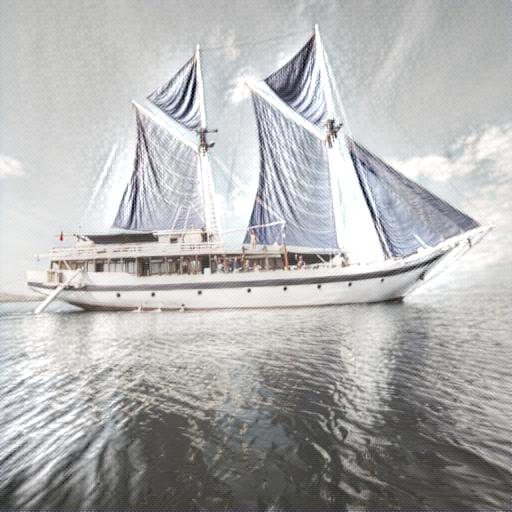
\includegraphics[width=0.19\textwidth]{style_transfer_ulyanov_a}\\
		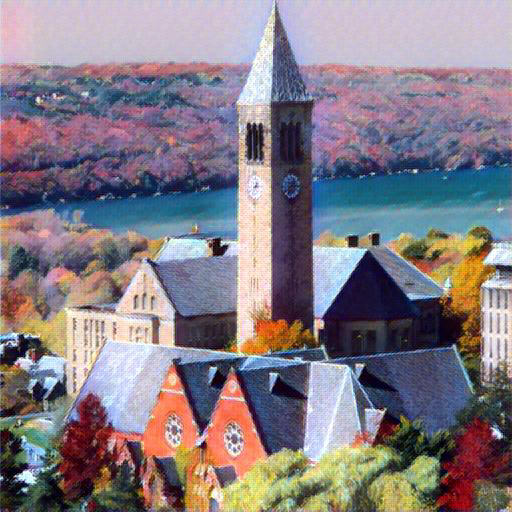
\includegraphics[width=0.19\textwidth]{style_transfer_ulyanov_b}\\
		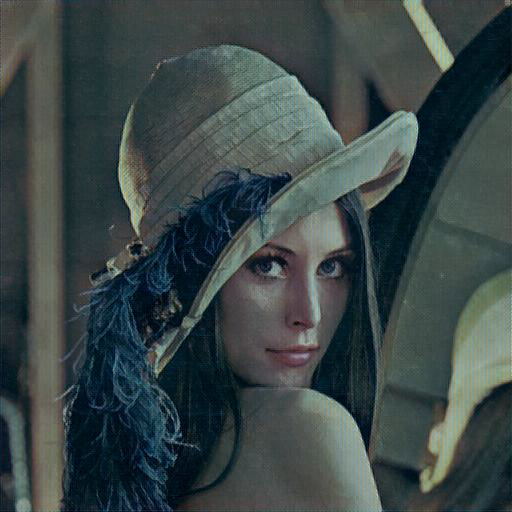
\includegraphics[width=0.19\textwidth]{style_transfer_ulyanov_c}\\
		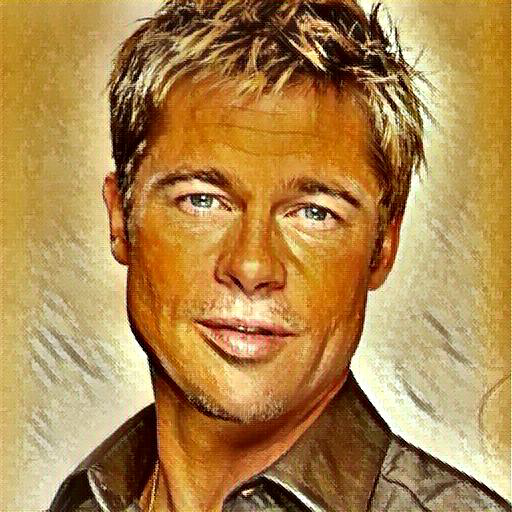
\includegraphics[width=0.19\textwidth]{style_transfer_ulyanov_d}\\
		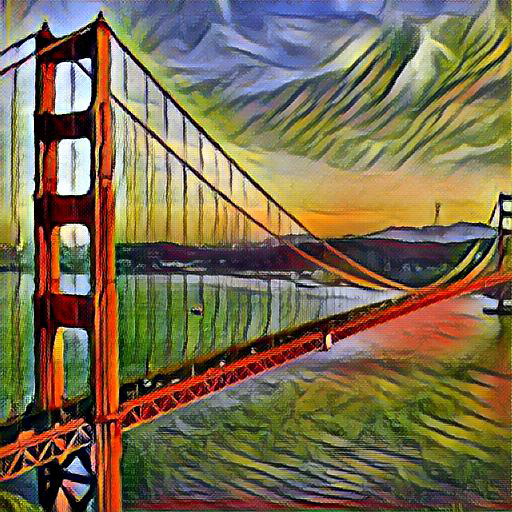
\includegraphics[width=0.19\textwidth]{style_transfer_ulyanov_e}\\
	}
	\subcaptionbox{Gatys et al.}[0.19\textwidth]{
		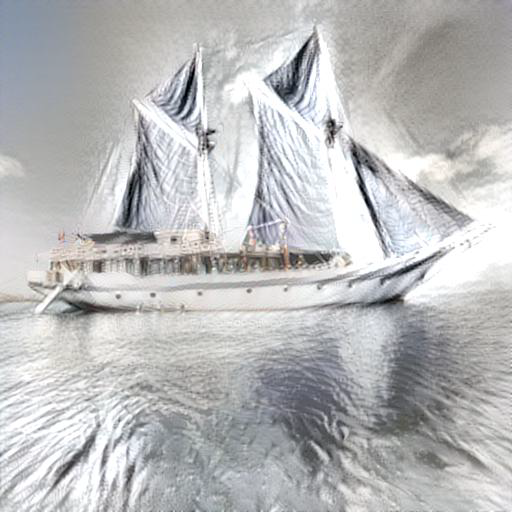
\includegraphics[width=0.19\textwidth]{style_transfer_gatys_a}\\
		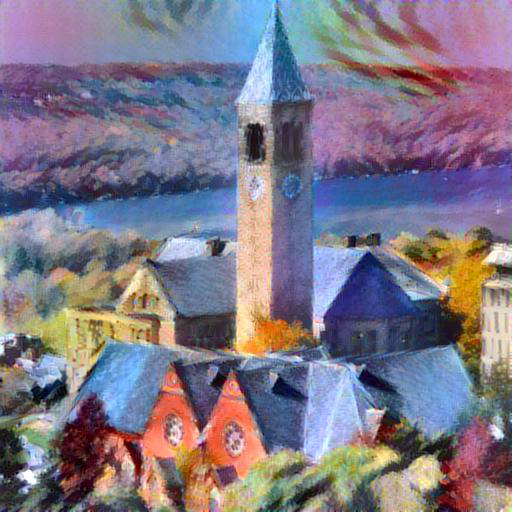
\includegraphics[width=0.19\textwidth]{style_transfer_gatys_b}\\
		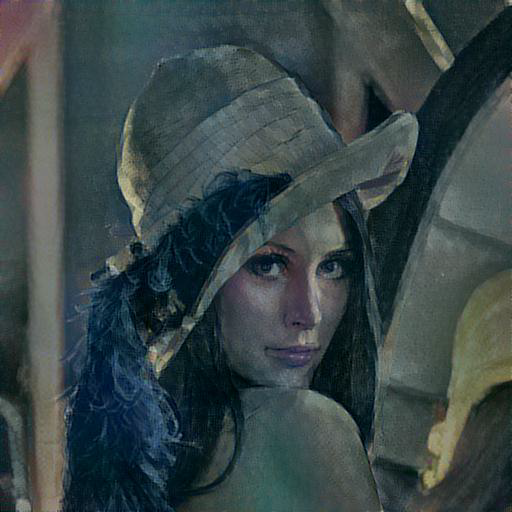
\includegraphics[width=0.19\textwidth]{style_transfer_gatys_c}\\
		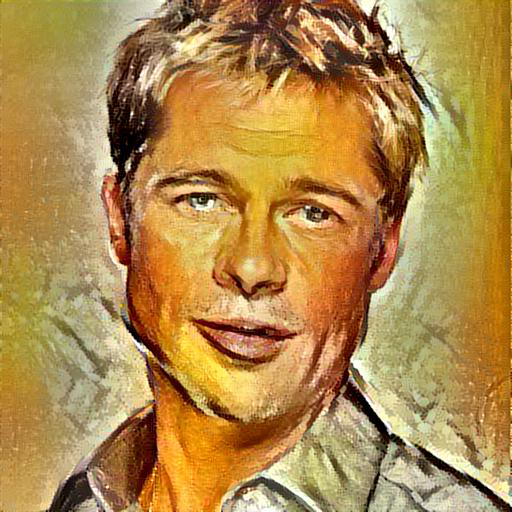
\includegraphics[width=0.19\textwidth]{style_transfer_gatys_d}\\
		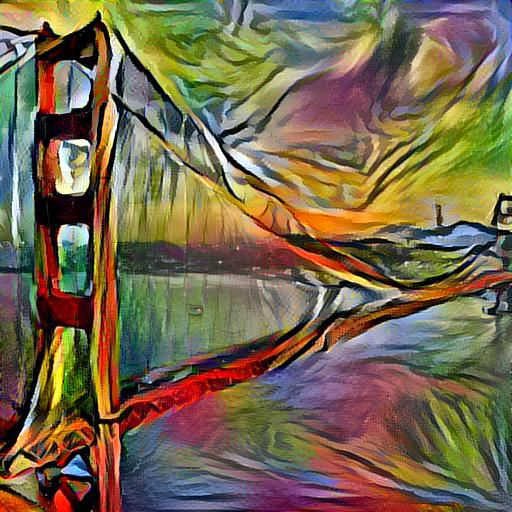
\includegraphics[width=0.19\textwidth]{style_transfer_gatys_e}\\
	}
	\caption{A comparison between different style transfers where the style was not seen during training.}
	\label{fig:style_transfer_unseen_style}
\end{figure}

\subsection{Generative Adversarial Networks}
With the introduction of \glspl{GAN}, the quality of generative models has greatly increased.
It is not surprising then that this got picked up in \gls{NST} research.
Among the first are Isola et al. \cite{Isola2016}, who use \gls{cGAN}.
They use the network from \cite{radford2016}, that uses modules of the form convolution-BatchNorm-ReLu\cite{Ioffe2015}.
Additionally, in order to pass shared features in the generator they add skip connections like with "U-Net" \cite{Ronneberger2015}.
For the discriminator, which they call PatchGAN, they validate $N\times N$ patches and take the average as output.
They take this loss together with the $L1$ loss because $L2$ loss produces blurry results.
However, this method still requires paired training samples.
Meanwhile, Taigman et al. \cite{Taigman2016} are doing research in unsupervised domain transfer.
Research in domain transfer can be easily adjusted for use in \gls{NST}, but this is not possible the other way around.
Their network uses an autoencoder as the generator and they assume that the encoder is fixed between domains.
The discriminator has a ternary output and distinguishes between real, fake and reconstruction.
They add several new loss functions which check the consistency between the two domains (consistency loss) and whether $G$ performs perfect reconstruction (reconstruction loss).
For the encoder, they use a pre-trained network that is trained on paired samples though.
In order to make the network completely unsupervised, Yi et al.\cite{Yi2017} propose DualGAN, Kim et al. \cite{Kim2017} DiscoGAN and Zhu et al. \cite{Zhu2017b} CycleGAN, which are all three essentially the same proposal.
The entire model consists of two cycle-consistent networks where each translates from one domain to the other.
A cycle-consistent network will first translate the input to a target domain and then back to the original domain.
Each domain has a discriminator which compares the real input from one network with the fake from the other; the adversarial loss.
In addition to this there's a cycle-consistency loss, which is the \gls{MSE} between the input and the reconstructed image as you can see in Figure \ref{fig:style_transfer_algorithm_cyclegan}.
The goal is to minimize the adversarial and cycle-consistency loss, while maximizing the discriminators' accuracy.

\begin{figure}[h]
	\centering
	\captionbox{
		\label{fig:style_transfer_algorithm_cyclegan}
		The cycle-consistent network by Zhu et al. \cite{Zhu2017b}.
		Unsupervised image-to-image translation between domains $X$ and $Y$ is established by training the generators $G$, $F$ and discriminators $D_X$, $D_Y$.
		During training cycle-consistency loss is calculated under the assumption that $F(G(x))\shouldeq x$ and $G(F(y))\shouldeq y$.
	}{	
		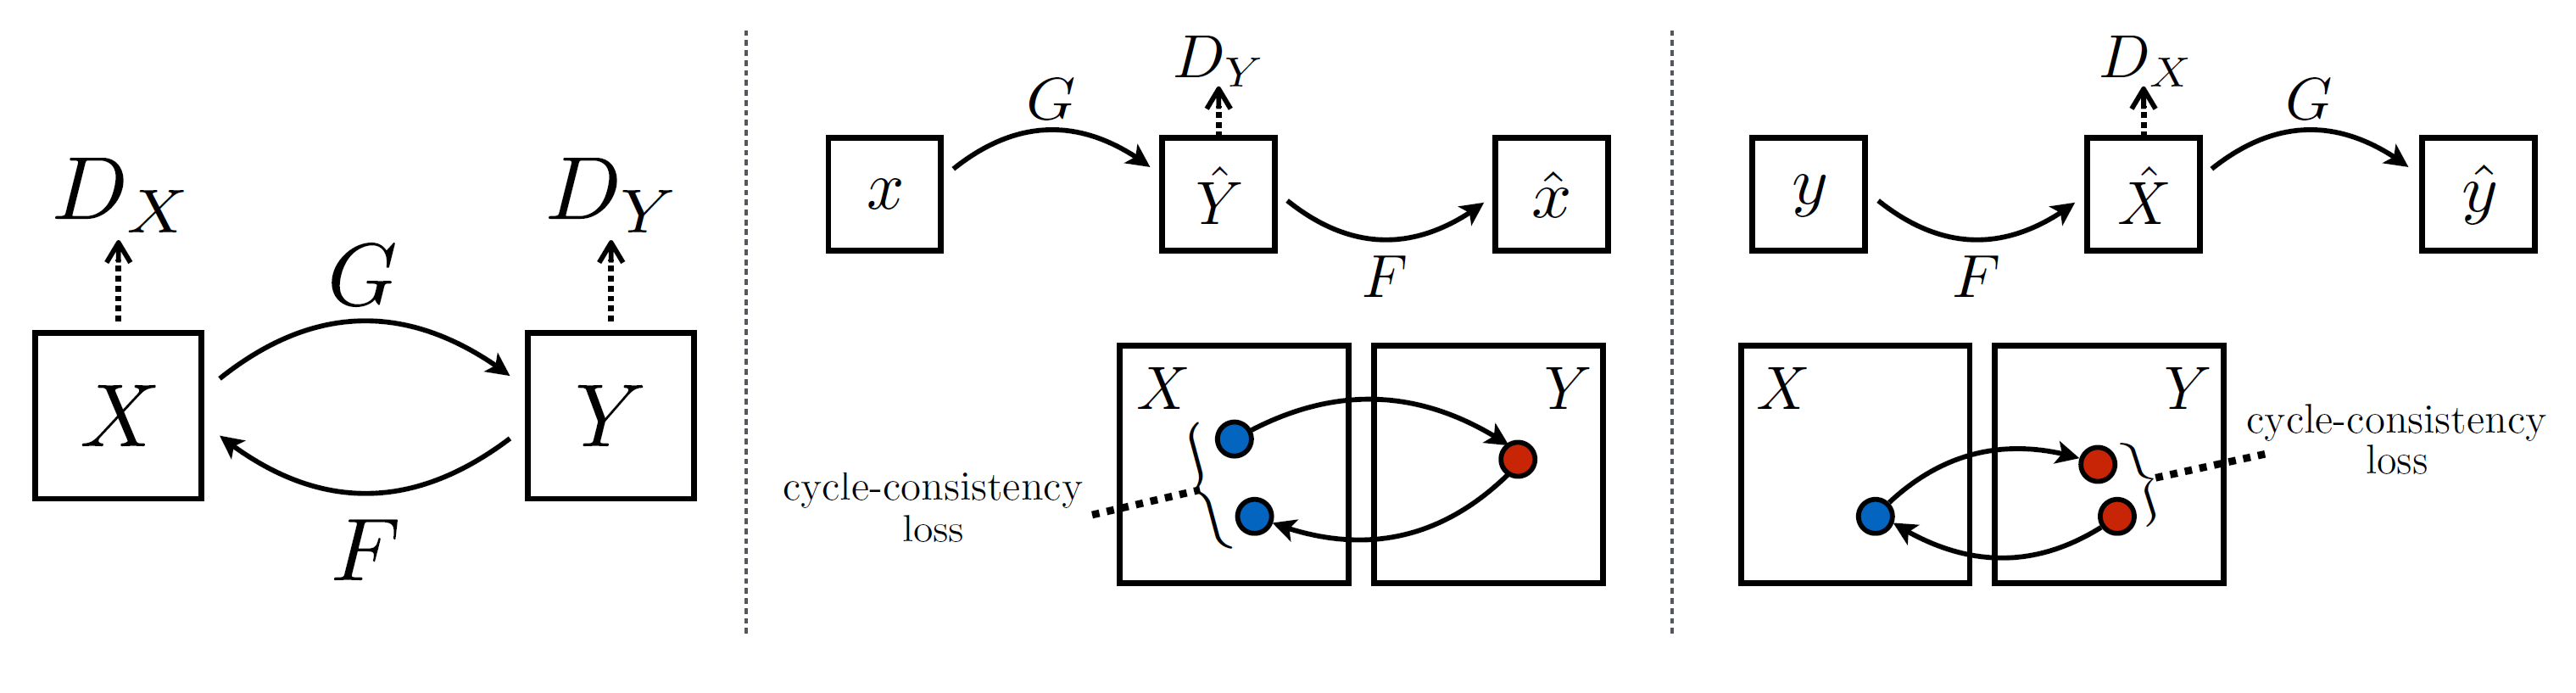
\includegraphics[width=\textwidth]{style_transfer_algorithm_cyclegan}%
	}
\end{figure}

Zhu et al. \cite{Zhu2017b} also introduce an identity loss.
Liu et al. \cite{Liu2017} introduce the latent space concept which assumes that paired images from different domains can be mapped to a shared latent space with the same latent representation.
Their network consists of two domain image encoders $E\textsubscript{$1$}$ and $E\textsubscript{$2$}$, two domain image generators $G\textsubscript{$1$}$ and $G\textsubscript{$2$}$, and two domain discriminators $D\textsubscript{$1$}$ and $D\textsubscript{$2$}$, as can be seen in \ref{fig:style_transfer_algorithm_unit}.
The encoders and generators are paired and form a \gls{VAE} \cite{kingma2022}.
The encoder maps the input to latent space, and the generator reconstructs the image.
This is the reconstruction loss.
They use weight-sharing, which shares the weight of the last two layers of the encoders and of the first two layers of the generators.
The generators and discriminators are paired to form a \gls{GAN}.
The generator can also construct an image from the latent code from the other encoder's input.
This image is used to train the \gls{GAN}.
They also show that the shared-latent space assumption implies cycle-consistency, which is the final loss function of the network.

\begin{figure}
	\centering
	\captionbox{
		\label{fig:style_transfer_algorithm_unit}
		Liu et al. \cite{Liu2017}.
	}{	
		\subcaptionbox{The shared latent space assumption.}[0.34\textwidth]{%
			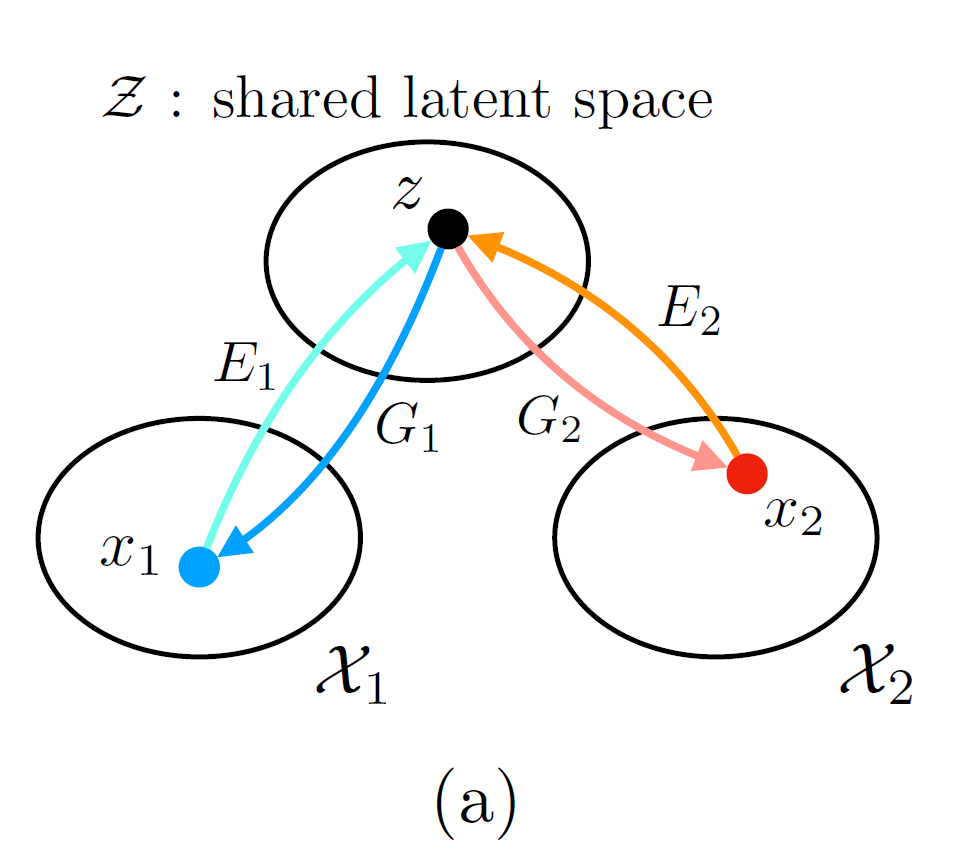
\includegraphics[width=0.34\textwidth]{style_transfer_algorithm_unit_a}%
		}
		\subcaptionbox{The unsupervised image-to-image translation network.}[0.64\textwidth]{%
			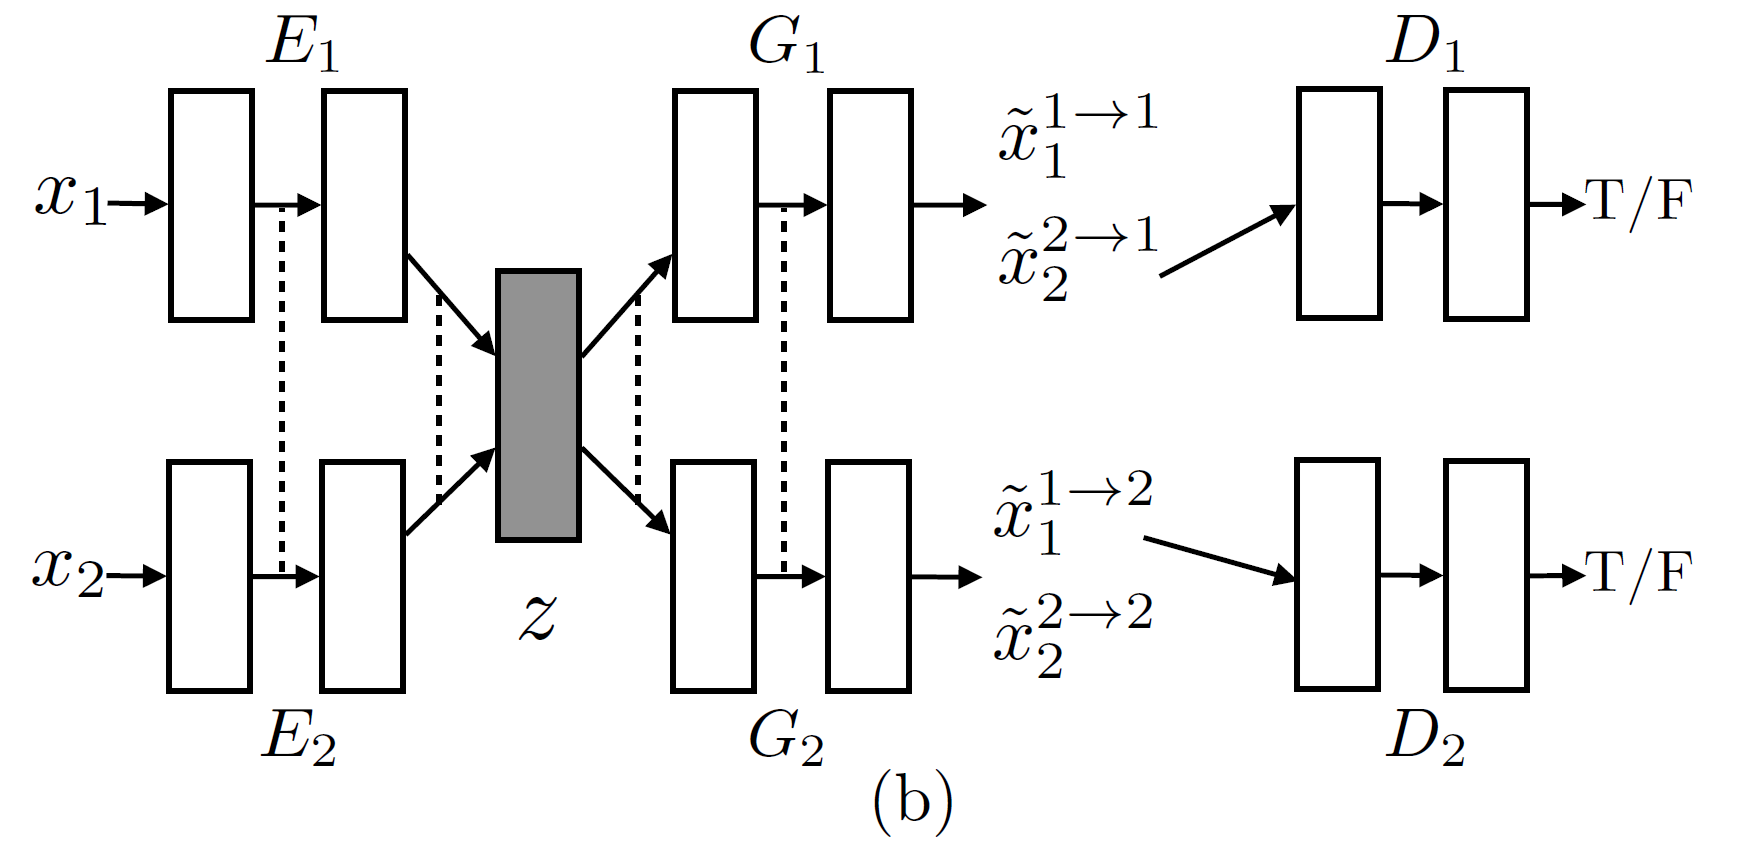
\includegraphics[width=0.64\textwidth]{style_transfer_algorithm_unit_b}%
		}
	}
\end{figure}

\subsection{Evaluation Metric}
\label{sec:style_transfer_metrics}
There are several methods to evaluate the quality of a generated image. 
A first metric is through human evaluation, where a score is given based on generation quality.
This proved to be inconsistent as a person's perception can change over time.
Afterwards, new metrics were introduced which will be discussed here. \cite{Hoyez2022}

\begin{enumerate}
	\item \textbf{\gls{PD}} is proposed by Johnson et al. \cite{Johnson2016}.
	It uses the VGG-16 network \cite{Simonyan2015} trained on ImageNet \cite{Deng2009} to define perceptual loss functions.
	These are extracted from the layers for the style and content images, and compared to the generated image.
	The lower the score, the better.
	\item \textbf{\gls{IS}}, as described by Salimans et al. \cite{Salimans2016}, uses a pre-trained Inception model \cite{Szegedy2015} to describe the quality of the generated images.
	It prescribes that the entropy of the distribution of predicted labels for individual images needs to be minimized while the entropy of the distribution across all images need to be high.
	This equates to each image having generated a distinct label and the labels being equally distributed.
	The closer to 1, the better.
	\item \textbf{\gls{FID}} is the most used measurement and suggested by Heusel et al. \cite{Heusel2017} to enhance \gls{IS}, because it is only calculated on the distribution of the generated images.
	\gls{FID} uses the Gaussian distribution of both real and generated images as it calculates the Fréchet distance \cite{Frechet1957} between them.
	The Gaussians are formed from the coding layer of the Inception network \cite{Szegedy2015}.
	The lower, the better.
	\item \textbf{\gls{LPIPS}} is a metric developed by Zhang et al. \cite{Zhang2018} and the second most popular.
	It calculates the distance between the activations of the hidden layers in an object detection model (several models are proposed).
	They show that this correlates closely to human perception.
	It can also be used to evaluate the diversity of a network by calculating the average \gls{LPIPS} score of a pair of randomly generated outputs.
	The higher, the better.
\end{enumerate}

\subsubsection{Summary}
There are plenty of other evaluation metrics available that also try to correlate closely to human evaluation, but they are mostly just attempts to improve previously discussed metrics.
Until this day, image similarity metrics continue to be a challenging problem.

\section{Content Based Image Retrieval}
\gls{CBIR}, a long-established research area, is the task of finding semantically matching or similar content images for a specified query image.
This has become increasingly relevant with the exponential growth of image and video data and the need to effectively search these image collections.
\gls{CBIR} has been used specifically for person re-identification, remote sensing, medical image search, and shopping recommendations in online marketplaces, among many others \cite{Chen2021a}.
Image retrieval can be categorized into two different groups: \gls{CIR} and \gls{IIR}.
\gls{CIR}'s goal is to find images within the same category as the query, while \gls{IIR} tries to find images with a particular instance given in the query image.
The general workflow of \gls{CBIR} is illustrated in \ref{fig:image_retrieval_flowchart}.
This thesis will only discuss query formation, image representation, image scoring, and search re-ranking.

\begin{figure}
	\centering
	\includegraphics[width=0.65\textwidth]{image_retrieval_flowchart}%
	\label{fig:image_retrieval_flowchart}
	\caption{
		The general workflow of Content Based Image Retrieval. \cite{Zhou2017}
	}
\end{figure}

\textbf{Query Formation} can be done several ways.
A user might want to find images based on keywords, which is your standard classification task.
Instead of just giving a series of keywords, these can also be arranged in a layout.
A query by concept layout will then search for an image with the same arrangement \cite{Xu2010}.
Similarly, a query by color layout will search for that arrangement of colors in the images \cite{Wang2011}.
It's also possible that a user wants to find images similar to a sketch (query by sketch) \cite{Cao2010} or another image (query by example) \cite{Radenovic2017}.
An overview can be found in Fig. \ref{fig:image_retrieval_query_formation}.

\begin{figure}[h]
	\centering
	\includegraphics[width=0.7\textwidth]{image_retrieval_query_formation}%
	\caption{
		An overview of the different kinds of queries with corresponding retrieval results. \cite{Zhou2017}
	}
	\label{fig:image_retrieval_query_formation}
\end{figure}

\textbf{Image Representation} is a major challenge with image retrieval.
It's goal is to proficiently measure similarity between images.
Clearly, directly comparing pixels values is impracticable, so methods that extract visual features from images are used.
They are transformed into a fixed-sized vector which form a representation of the image.
Before deep learning, hand crafted feature algorithms were used.
From these, \gls{SIFT} \cite{Lowe1999} was the most popular.
Thousands of features can be extracted this way, which is too much for an efficient query response.
These features are further compressed for which various methods exist, called feature aggregation.

\textbf{Image scoring} gives the results during a search a relevance score for ranking.
This score is determined by one of two ways:
During feature aggregation, the image is represented with a fixed-sized vector.
The relevance can be calculated with the $L_p$-normalized distance between the feature aggregation vectors.
Scoring can also be quantified based on voting.
This can be achieved by counting each similar feature to the vote \cite{Zhou2011}, or through the calculation of \gls{TF-IDF} \cite{Zhang2011}.

\textbf{Search Reranking} are post-processing techniques that improve the accuracy of the query.
Among them is geometric context verification, which will try to eliminate false similarities by looking at geometric context, like rotation, scale and the relations between local features.
Another is to reuse the highest ranked results to create new queries which can expand on the original.
Missed features in the original query can be found this way and improve recall performance.
As a last improvement, different retrieval techniques can be merged together to give better results with retrieval fusion.

The model used in this work, by Radenovic et al. \cite{Radenovic2017}, trains a VGG network from reconstructed 3D models obtained by retrieval and structure-from-motion methods.
This allows them to use the geometry and camera positions to enhance the feature extraction along with several other optimization techniques.
During training, they make use of the contrastive loss.
Contrastive loss is minimized when similar image pairs are close to each other in embedding space and different pairs are far away.

\section{Deep learning in the Art domain}
\label{sec:related_papers}
Various papers have already discussed different techniques to improve object detection and pose estimation on artworks.
In this section, three of those papers will be discussed.
One paper discusses how the digitization of artworks can benefit the analysis of art collections.
The other two discuss techniques of how existing models can be adapted to work on art collections.
\\

Through digitization, analysis of art collections has become more efficient.
Artists are constantly inspiring and being inspired, and in order to correctly analyze the relation between paintings and artists, it's beneficial to have a method that finds their inspirations.
One way that can be achieved is by using image retrieval, which gives good results, but only when the works are visually similar, like with religious paintings.
In other cases, the inspiration is drawn from themes, which involve composition, lighting and poses.
Jenicek et al. \cite{Jenicek2019} propose finding these relations by analyzing the similarity between poses.
From a database of images the poses are estimated and normalized.
They then employ a two step process: with a query image and fast matching, they generate a shortlist of possible hits.
Afterwards, geometric validation filters out impossible alignments with the query image.
Their experiments show significant improvements over previous methods.
They also note some failure cases where pose estimation falls short, like failing to find keypoints or making associations with wrong poses.
\\
\\

\begin{figure}[h]
	\centering
	\captionbox{
		\label{fig:related_papers_madhu}
		Improvements to the state-of-the-art by Madhu et al. \cite{Madhu2020}.
	}{	
		\subcaptionbox{Original}[0.20\textwidth]{%
			\includegraphics[width=0.20\textwidth]{related_papers_vase}%
		}
		\subcaptionbox{OpenPose}[0.20\textwidth]{%
			\includegraphics[width=0.20\textwidth]{related_papers_vase_sota}%
		}
		\subcaptionbox{Madhu et al.}[0.20\textwidth]{%
			\includegraphics[width=0.20\textwidth]{related_papers_vase_stl}%
		}
	}
\end{figure}

To improve these shortcomings on Greek vases, Madhu et al. \cite{Madhu2020} apply style transfer to the COCO dataset with AdaIN in the style of those vases and use this for fine-tuning.
They use a top-down architecture with Faster R-CNN as detector and HRNet for pose estimation.
They also created their own small dataset to evaluate their improvements (Figure \ref{fig:related_papers_madhu}).
Kadish et al. \cite{Kadish2021} have the same idea and also use AdaIN to stylize the COCO dataset.
They randomly sample artworks from the Painter by Numbers dataset from Kaggle \cite{PainterByNumbers} for the style images and using it to fine-tune the Faster R-CNN network for object detection.
Both papers found an improvement in the performance of the networks on art collections, which is further discussed in Section \ref{sec:improvements_related_papers}.
\\

Part of this thesis will combine the previously discussed work.
While Madhu et al. only fine-tuned a network to work better for Greek vases, it would be more useful if the fine-tuned model could be used more generally.
This is what Kadish et al. achieve, but they focused on the object detection task.
Here, both methods will be combined to achieve improvements in pose estimation on non-specific art collections.